\documentclass[letter,12pt,oneside,spanish]{ezthesis}

%% # Opciones disponibles para el documento #
%%
%% Las opciones con un (*) son las opciones predeterminadas.
%%
%% Modo de compilar:
%%   draft            - borrador con marcas de fecha y sin im'agenes
%%   draftmarks       - borrador con marcas de fecha y con im'agenes
%%   final (*)        - version final de la tesis
%%
%% Tama'no de papel:
%%   letterpaper (*)  - tama'no carta (Am'erica)
 %%   a4paper          - tama'no A4    (Europa)
%%
%% Formato de impresi'on:
%%   oneside          - hojas impresas por un solo lado
%%   twoside (*)      - hijas impresas por ambos lados
%%
%% Tama'no de letra:
%%   10pt, 11pt, o 12pt (*)
%%
%% Espaciado entre renglones:
%%   singlespace      - espacio sencillo
%%   onehalfspace (*) - espacio de 1.5
%%   doublespace      - a doble espacio
%%
%% Formato de las referencias bibliogr'aficas:
%%   numbers          - numeradas, p.e. [1]
%%   authoryear (*)   - por autor y a'no, p.e. (Newton, 1997)
%%
%% Opciones adicionales:
%%   spanish         - tesis escrita en espa'nol
%%
%% Desactivar opciones especiales:
%%   nobibtoc   - no incluir la bibiolgraf'ia en el 'Indice general
%%   nofancyhdr - no incluir "fancyhdr" para producir los encabezados
%%   nocolors   - no incluir "xcolor" para producir ligas con colores
%%   nographicx - no incluir "graphicx" para insertar gr'aficos
%%   nonatbib   - no incluir "natbib" para administrar la bibliograf'ia

%% Paquetes adicionales requeridos se pueden agregar tambi'en aqu'i.
%% Por ejemplo:
%%\usepackage[spanish]{babel}
\usepackage[utf8]{inputenc}
\usepackage[all]{xy}
\usepackage{colortbl}
\usepackage[sort&compress,round,authoryear]{natbib}
\usepackage{longtable}
\usepackage{multirow, array}
\usepackage{graphicx} 
\usepackage{float} 
\usepackage{pgfgantt} 
\usepackage{enumerate}


%% # Datos del documento #
%%\documentclass[12pt]{•}%% Nota que los acentos se deben escribir: \'a, \'e, \'i, etc.
%% La letra n con tilde es: \~n.

% para los colores en las referencias
\usepackage[colorlinks=true,linkcolor=black,citecolor=blue,filecolor=red,pagecolor=cyan,urlcolor=cyan]{hyperref}

\author{Stephanie Katherine Correa Alc\'antara}
\title{Desarrollo de una aplicaci\'on Web para el estudio de datos longitudinales para el seguimiento de la infecci\'on por el Virus de Inmunodeficiencia Humana, caso de estudio: Instituto Aut\'onomo Hospital Universitario de los Andes}
\degree{Ingeniero en Inform\'atica}
\supervisor{ Rossana Timaure Garc\'ia. PhD.}
\institution{Universidad Nacional Experimental del T\'achira}
\faculty{Vicerrectorado Acad\'emico}
\department{Departamento de Ingenier\'ia en Inform\'atica}

%% # M'argenes del documento #
%% 
%% Quitar el comentario en la siguiente linea para austar los m'argenes del
%% documento. Leer la documentaci'on de "geometry" para m'as informaci'on.

\geometry{left=3cm,right=3cm,top=4cm,bottom=3cm}

%% El siguiente comando agrega ligas activas en el documento para las
%% referencias cruzadas y citas bibliogr'aficas. Tiene que ser *la 'ultima*
%% instrucci'on antes de \begin{document}.
%%\hyperlinking
\begin{document}

%% En esta secci'on se describe la estructura del documento de la tesis.
%% Consulta los reglamentos de tu universidad para determinar el orden
%% y la cantidad de secciones que debes de incluir.

%% # Portada de la tesis #
%% Mirar el archivo "titlepage.tex" para los detalles.
%% ## Construye tu propia portada ##
%% 
%% Una portada se conforma por una secuencia de "Blocks" que incluyen
%% piezas individuales de informaci'on. Un "Block" puede incluir, por
%% ejemplo, el t'itulo del documento, una im'agen (logotipo de la universidad),
%% el nombre del autor, nombre del supervisor, u cualquier otra pieza de
%% informaci'on.
%%
%% Cada "Block" aparece centrado horizontalmente en la p'agina y,
%% verticalmente, todos los "Blocks" se distruyen de manera uniforme 
%% a lo largo de p'agina.
%%
%% Nota tambi'en que, dentro de un mismo "Block" se pueden cortar
%% lineas usando el comando \\
%%
%% El tama'no del texto dentro de un "Block" se puede modificar usando uno de
%% los comandos:
%%   \small      \LARGE
%%   \large      \huge
%%   \Large      \Huge
%%
%% Y el tipo de letra se puede modificar usando:
%%   \bfseries - negritas
%%   \itshape  - it'alicas
%%   \scshape  - small caps
%%   \slshape  - slanted
%%   \sffamily - sans serif
%%
%% Para producir plantillas generales, la informaci'on que ha sido inclu'ida
%% en el archivo principal "tesis.tex" se puede accesar aqu'i usando:
%%   \insertauthor
%%   \inserttitle
%%   \insertsupervisor
%%   \insertinstitution
%%   \insertdegree
%%   \insertfaculty
%%   \insertdepartment
%%   \insertsubmitdate

\begin{titlepage}
\vspace*{-4cm}
  \TitleBlock{
\includegraphics[scale=0.2]{unet.jpg} }  
  \TitleBlock{\small\insertinstitution}
  \TitleBlock[\small]{\insertfaculty}
  \TitleBlock[\small]{Decanato de Docencia}
  \TitleBlock[\small]{\insertdepartment}
  \TitleBlock[\small]{Trabajo de Aplicaci\'on Profesional}
  \TitleBlock[\small]{Proyecto Especial de Grado}
  \vspace*{3cm}
    
 \TitleBlock{\scshape\inserttitle}
 
 \vspace*{3cm}
 
 \begin{flushright}
  \TitleBlock[\small]{ Autor: \insertauthor} 
  \TitleBlock[\small]{C.I.: V-19.598.574}
  \TitleBlock[\small]{stephanie.correa24@gmail.com}
  \TitleBlock[\small]{Tutor: \insertsupervisor}
  \TitleBlock[\small]{rttg@unet.edu.ve}
 \end{flushright}
  \TitleBlock{\small San Crist\'obal, Julio de 2018}
  
\end{titlepage}

%% Nota 1:
%% Se puede agregar un escudo o logotipo en un "Block" como:
%%   \TitleBlock{\includegraphics[height=4cm]{escudo_uni}}
%% y teniendo un archivo "escudo_uni.pdf", "escudo_uni.png" o "escudo_uni.jpg"
%% en alg'un lugar donde LaTeX lo pueda encontrar.

%% Nota 2:
%% Normalmente, el espacio entre "Blocks" se extiende de modo que el
%% contenido se reparte uniformemente sobre toda la p'agina. Este
%% comportamiento se puede modificar para mantener fijo, por ejemplo, el
%% espacio entre un par de "Blocks". Escribiendo:
%%   \TitleBlock{Bloque 1}
%%   \TitleBlock[\bigskip]{Bloque2}
%% se deja un espacio "grande" y de tama~no fijo entre el bloque 1 y 2.
%% Adem'as de \bigskip est'an tambi'en \smallskip y \medskip. Si necesitas
%% aun m'as control puedes usar tambi'en, por ejemplo, \vspace*{2cm}.



%% ## Construye tu propia portada ##
%% 
%% Una portada se conforma por una secuencia de "Blocks" que incluyen
%% piezas individuales de informaci'on. Un "Block" puede incluir, por
%% ejemplo, el t'itulo del documento, una im'agen (logotipo de la universidad),
%% el nombre del autor, nombre del supervisor, u cualquier otra pieza de
%% informaci'on.
%%
%% Cada "Block" aparece centrado horizontalmente en la p'agina y,
%% verticalmente, todos los "Blocks" se distruyen de manera uniforme 
%% a lo largo de p'agina.
%%
%% Nota tambi'en que, dentro de un mismo "Block" se pueden cortar
%% lineas usando el comando \\
%%
%% El tama'no del texto dentro de un "Block" se puede modificar usando uno de
%% los comandos:
%%   \small      \LARGE
%%   \large      \huge
%%   \Large      \Huge
%%
%% Y el tipo de letra se puede modificar usando:
%%   \bfseries - negritas
%%   \itshape  - it'alicas
%%   \scshape  - small caps
%%   \slshape  - slanted
%%   \sffamily - sans serif
%%
%% Para producir plantillas generales, la informaci'on que ha sido inclu'ida
%% en el archivo principal "tesis.tex" se puede accesar aqu'i usando:
%%   \insertauthor
%%   \inserttitle
%%   \insertsupervisor
%%   \insertinstitution
%%   \insertdegree
%%   \insertfaculty
%%   \insertdepartment
%%   \insertsubmitdate

\begin{titlepage}
\vspace*{-4cm}
  \TitleBlock{
\includegraphics[scale=0.2]{unet.jpg} }  
  \TitleBlock{\small\insertinstitution}
  \TitleBlock[\small]{\insertfaculty}
  \TitleBlock[\small]{Decanato de Docencia}
  \TitleBlock[\small]{\insertdepartment}
  \TitleBlock[\small]{Trabajo de Aplicaci\'on Profesional}
  \TitleBlock[\small]{Proyecto Especial de Grado}
  \vspace*{3cm}
    
 \TitleBlock{\scshape\inserttitle}
 {\small  Proyecto especial de grado presentado como requisito parcial para optar al t\'itulo de Ingeniero en Inform\'atica}
 \vspace*{2cm}
 
 \begin{flushright}
  \TitleBlock[\small]{ Autor: \insertauthor} 
  \TitleBlock[\small]{C.I.: V-19.598.574}
  \TitleBlock[\small]{stephanie.correa24@gmail.com}
  \TitleBlock[\small]{Tutor: \insertsupervisor}
  \TitleBlock[\small]{rttg@unet.edu.ve}
 \end{flushright}
  \TitleBlock{\small San Crist\'obal, Julio de 2018}
  
\end{titlepage}

%% Nota 1:
%% Se puede agregar un escudo o logotipo en un "Block" como:
%%   \TitleBlock{\includegraphics[height=4cm]{escudo_uni}}
%% y teniendo un archivo "escudo_uni.pdf", "escudo_uni.png" o "escudo_uni.jpg"
%% en alg'un lugar donde LaTeX lo pueda encontrar.

%% Nota 2:
%% Normalmente, el espacio entre "Blocks" se extiende de modo que el
%% contenido se reparte uniformemente sobre toda la p'agina. Este
%% comportamiento se puede modificar para mantener fijo, por ejemplo, el
%% espacio entre un par de "Blocks". Escribiendo:
%%   \TitleBlock{Bloque 1}
%%   \TitleBlock[\bigskip]{Bloque2}
%% se deja un espacio "grande" y de tama~no fijo entre el bloque 1 y 2.
%% Adem'as de \bigskip est'an tambi'en \smallskip y \medskip. Si necesitas
%% aun m'as control puedes usar tambi'en, por ejemplo, \vspace*{2cm}.



%%\include{autorizacion}
%%\chapter*{}
\pagestyle{empty}
\thispagestyle{empty}
\vspace*{-4cm}
\begin{figure}[H]
\includegraphics[scale=0.22]{aprobacion_Tap.JPG}
\end{figure}

%% # Prefacios #
%% Por cada prefacio (p.e. agradecimientos, resumen, etc.) crear
%% un nuevo archivo e incluirlo aqu'i.
%% Para m'as detalles y un ejemplo mirar el archivo "gracias.tex".

\addcontentsline{toc}{chapter}{Dedicatoria}
\cleardoublepage
\chapter*{Dedicatoria}
\pagenumbering{Roman}

\begin{flushright}
\textit{A Dios todopoderoso.\\
A mis padres.\\
A mi pequeño Mart\'in valiente.\\
A Daniel.\\ 
Y a la UNET}
\end{flushright}
\addcontentsline{toc}{chapter}{Agradecimientos}
\cleardoublepage

\chapter*{Agradecimientos}


Primeramente  a Dios, por darme la salud y fortaleza, porque me ha gu\'iado e iluminado a lo largo de mi vida, especialmente para alcanzar esta meta.\\

A mis padres, Magalys y Rafael, por todo el indudable apoyo econ\'omico y moral en todo momento, por escucharme, por confiar y tener esperanza en m\'i.\\

A Daniel, por su amor, comprensi\'on y paciencia en los momentos en los que m\'as he necesitado. \\

A mi hijo Mart\'in, el cual representa mi orgullo y mi motivaci\'on principal para ser una mejor persona y servirle de ejemplo.\\

A toda mi familia en general, por el apoyo brindado a lo largo de los años.\\

A la tutora, Rossana Timaure, por darme la oportunidad, apoyo y conocimientos para la realizaci\'on de este trabajo de grado.\\

A todos los profesores que a lo largo de la carrera me brindaron la gu\'ia necesaria y el conocimiento.\\

A la ilustre Universidad Nacional Experimental del T\'achira, por permitirme entrar en sus aulas y formarme como profesional.

\addcontentsline{toc}{chapter}{Resumen}
\cleardoublepage
\chapter*{}
\pagestyle{empty}
\thispagestyle{empty}

\begin{center}
\vspace*{-4cm}
Universidad Nacional Experimental del T\'achira\\
Vicerrectorado Acad\'emico\\
Decanato de Docencia\\
Departamento de Ingenier\'ia Inform\'atica\\

\end{center}
\begin{center}
\textbf{Desarrollo de una aplicaci\'on Web para el estudio de datos longitudinales para el seguimiento de la infecci\'on por el Virus de Inmunodeficiencia Humana, caso de estudio: Instituto Aut\'onomo Hospital Universitario de los Andes}
\end{center}
\begin{flushright}
Autor: Correa Alc\'antara, Stephanie Katherine \\
Tutor:  Timaure Garc\'ia, Rossana. PhD. \\
Fecha: Julio 2018.\\
\end{flushright}

\small{
\begin{center}
\textbf{RESUMEN}
\end{center}

\noindent
Se describe el desarrollo de una aplicaci\'on web como paquete del lenguaje de programaci\'on R,  para el seguimiento de la infecci\'on por el virus de inmunodeficiencia humana (VIH), haciendo uso de datos longitudinales y el modelo lineal mixto. La metodolog\'ia de desarrollo de  \textit{software} empleada fue la espiral, mediante la cual se realiz\'o el filtrado, descripción y exploraci\'on de la base de datos del Laboratorio de Investigaciones Hormonales de Instituto Aut\'onomo Hospital Universitario de los Andes, en la cual se almacena la informaci\'on de seguimiento del comportamiento de los biomarcadores de los pacientes pertenecientes al Programa Nacional SIDA/ITS, de aqu\'i se obtuvieron las vistas minables que sirvieron para determinar el formato de los datos de entrada a la aplicaci\'on;  de igual forma se contruyeron y codificaron los modelos de funciones que integran el paquete, utilizando la dependencia con el paquete  \textit{Shiny} de R para el despliegue gr\'afico sobre el mapa de Venezuela de las caracter\'isticas demogr\'aficas y densidad de los pacientes registrados en la base de datos, as\'i como se implemento una funci\'on para el ajuste y estimaci\'on de un modelo lineal de efectos mixtos, que permita explorar de forma descriptiva, que factores resultan significativos para explicar la variabilidad de la carga viral plasm\'atica \'o el conteo de c\'elulas $T^{+}CD4$. \\

\noindent
\textbf{Palabras clave:} Datos longitudinales, modelo lineal mixto, VIH, R, Shiny.
}



%\chapter*{}
\pagestyle{empty}
\thispagestyle{empty}
\begin{flushright}
\vspace*{-4cm}
San Crist\'obal, Marzo de 2017
\end{flushright}

\vspace*{1cm}
\begin{flushleft}
Se\~nores:
\textbf{Miembros de la Comisi\'on de Trabajo de Aplicaci\'on profesional}
Departamento de Ingenier\'ia Inform\'atica
\end{flushleft}

\vspace*{1cm}

	Yo, Stephanie Katherine Correa Alc\'antara, titular de la c\'edula de identidad N V-19.598.574, inscrita en el per\'iodo acad\'emico 2017-1, estudiante del noveno semestre de Ingenier\'ia Inform\'atica, por medio de la presente, someto a consideraci\'on de la Comisi\'on de Trabajo de Aplicaci\'on Profesional de este Departamento la propuesta de Proyecto Especial de Grado titulado: \textbf{Desarrollo de una aplicaci\'on Web para el estudio de datos longitudinales para el seguimiento de la infecci\'on por el Virus de Inmunodeficiencia Humana, caso de estudio: Instituto Aut\'onomo Hospital Universitario de los Andes}, la cual se desarrollar\'a bajo la tutor\'ia de la profesora: Rossana Timaure.\\
	
	
	Se anexan los recaudos exigidos, de acuerdo con lo dispuesto en la normativa para el Trabajo de Aplicaci\'on Profesional de la Universidad Nacional Experimental del T\'achira. La fecha estimada de culminaci\'on del  proyecto: 26/06/2017
	\\
	
	Sin otro particular a que hacer referencia y en espera de su respuesta,\\
	
	
	Atentamente,\\
	
	\vspace*{2cm}
	
	\begin{center}
	
	Stephanie Katherine Correa Alc\'antara
	
	C.I. V-19.598.574
	\end{center}
	 
%\include{aprobacion}

%% # 'Indices y listas de contenido #
%% Quitar los comentarios en las lineas siguientes para obtener listas de
%% figuras y cuadros/tablas.
\pagenumbering{roman}
\setcounter{page}{4} 
\cleardoublepage
\addcontentsline{toc}{chapter}{\'Indice General}
\tableofcontents
\renewcommand{\listtablename}{\'Indice de Cuadros}
\cleardoublepage
\addcontentsline{toc}{chapter}{\'Indice de Cuadros} % para que aparezca en el indice de contenidos
\listoftables % indice de tablas
\cleardoublepage
\addcontentsline{toc}{chapter}{\'Indice de Figuras} % para que aparezca en el indice de contenidos
\listoffigures % indice de figuras
\cleardoublepage


%% # Cap'itulos #
%% Por cada cap'itulo hay que crear un nuevo archivo e incluirlo aqu'i.
%% Mirar el archivo "intro.tex" para un ejemplo y recomendaciones para
%% escribir.
%%\cleardoublepage
\pagenumbering{arabic}
\addcontentsline{toc}{chapter}{Introducci\'on}
%%\markboth{Introducci\'on}{Introducci\'on} % encabezado 

\chapter*{Introducci\'on}
\pagenumbering{arabic} % para empezar la numeración con números

El \textit{software} R es un entorno de c\'odigo abierto para la computaci\'on y graficaci\'on estad\'istica. El \textit{software} se compila y ejecuta en Windows, Mac OS X y Linux, distribuy\'endose usualmente en formato binario para facilitar su instalaci\'on. El proyecto de \textit{software} R fue iniciado por Robert Gentleman y Ross Ihaka. En R, la unidad fundamental de c\'odigo compartible es el paquete o la librer\'ia, el cual agrupa c\'odigo, datos, documentaci\'on y pruebas, y resulta simple de compartir con otros. Para enero del 2015 ya hab\'ian m\'as de 6.000 paquetes disponibles en la Red Integral de Archivos de R, conocido com\'unmente por su acr\'onimo CRAN, el cual es el repositorio de paquetes. Esta gran variedad de paquetes es una de las razones por las cuales R es tan exitoso, pues es probable que alg\'un investigador o acad\'emico ya haya resuelto un problema en su propio campo usando esta herramienta, por lo que otros usuarios simplemente podr\'an recurrir a ella para su uso directo o para llamarla en un nuevo c\'odigo.\\

	El diagn\'ostico de una enfermedad basado en la historia cl\'inica presentada por el paciente es un proceso complejo, involucra s\'intomas espec\'ificos as\'i como estudios realizados y afecciones presentadas en el tiempo. Una de las enfermedades con m\'as incidencia en la humanidad ha sido el Virus de Inmunodeficiencia Humana (VIH), el agente al entrar en el torrente sangu\'ineo por cualquiera de las formas de transmisi\'on, provoca un proceso de infecci\'on, en cierto tipo de c\'elulas del sistema inmunol\'ogico. Estas c\'elulas generan anticuerpos producidos como una reacci\'on de contraataque ante la presencia del VIH,  como los linfocitos $T^{+}CD4$; seg\'un los an\'alisis cl\'inicos dichas c\'elulas deb\'en estar en un rango normal de 500 a 1600 c\'elulas por mil\'imetro cubico de sangre ($mm^{3}$). Cuando estas cifras bajan significativamente a 200 c\'elulas de $T^{+}CD4$ por cada $mm^{3}$ de sangre, se dice que el sistema inmunol\'ogico est\'a muy d\'ebil indicando el desarrollo del Sindrome de Inmunodeficiencia Adquirida (SIDA).\\  

	En ese orden de ideas, la epidemia del VIH presenta muchos factores de gran inter\'es para ser estudiados y analizados bajo un enfoque temporal. En tal sentido, en el estudio epidemiol\'ogico se tiene como objetivo principal descifrar las relaciones que representan las variables persona y tiempo; este \'ultimo muchas veces no es considerado importante por lo tanto implica su estudio, dichas razones dan espacio para el an\'alisis del patr\'on temporal en eventos de salud sea fundamental para entender la exposici\'on al virus y prevenir eventos en el futuro, m\'as all\'a de si el proceso es contagioso, influenciado por el ambiente o relacionado a la variabilidad genot\'ipica. \\
	
	Desde el punto de vista temporal, la epidemiolog\'ia aporta grandes aspectos como lo son la determinaci\'on de los factores y los marcadores biol\'ogicos asociados a la progresi\'on y la efectividad de los tratamientos en la enfermedad, a lo largo del tiempo, por ende es de gran importancia en el enfoque para el estudio de datos longitudinales para el seguimiento de la infecci\'on \\

	La metodolog\'ia de investigaci\'on a aplicar es la de desarrollo de software en espiral, la cual consiste en la evaluaci\'on  de  los riesgos establecidos previamente en la planificaci\'on  y el an\'alisis de los datos por utilizar, en esta ocasi\'on son representativos de cada uno de los valores expuestos y obtenidos a trav\'es de ex\'amenes cl\'inicos realizados a cada uno de los pacientes en un determinado per\'iodo, dicha investigaci\'on  refleja un gran aporte cient\'ifico y m\'edico, con un enorme grado de importancia para la medicina, por lo tanto actualmente no se utiliza ning\'un sistema para el manejo y an\'alisis de datos. \\

	No obstante en cada uno de los cap\'itulos que conforman esta investigaci\'on, se expone y describe de forma detallada el problema del caso de estudio, el objetivo principal y espec\'ificos, la justificaci\'on y su alcance, acompa\~nados con el marco te\'orico, englobando todos aquellos conceptos y teor\'ias indispensables para la mejor comprensi\'on del tema, como tambi\'en el apartado metodol\'ogico empleado y el cual se llev\'o a cabo para la completa resoluci\'on de la investigaci\'on, por \'ultimo el desarrollo y ejecuci\'on del proyecto.

\chapter{El problema}

\section{Planteamiento y formulaci\'on}

Actualmente todas las organizaciones se ven forzadas al uso de la tecnolog\'ia como herramienta para desenvolverse con mayor eficiencia y eficacia en el desempe\~no de sus funciones. En la gesti\'on de la salud, la evaluaci\'on cl\'inica de los pacientes genera una serie de informaci\'on m\'edica y administrativa sobre los mismos. Esta informaci\'on a su vez, se registra en varios documentos f\'isicos o en formato digital, siendo el conjunto de \'estos lo que constituye la historia cl\'inica. \\

En los hospitales y centros cl\'inicos ambulatorios del Estado M\'erida, as\'i como en los diversos establecimientos de salud del pa\'is, la historia m\'edica es un componente b\'asico en el registro y seguimiento de los pacientes, as\'i pues se tratan en dichas instituciones; por ende este componente debe ser una herramienta de trabajo, garantizando el adecuado tratamiento de todos los pacientes. \\

No obstante, tanto el incremento del uso de la tecnolog\'ia y su evoluci\'on no son m\'otivo suficiente para justificar el uso de esta aplicaci\'on, hay razones importantes, como lo es el optimizar la b\'usqueda de informaci\'on registrada en el tiempo, acerca de una enfermedad o s\'intoma entre otros t\'opicos, ya pues en muchas ocasiones la informaci\'on obtenida no se encuentra almacenada en varios formatos o medios para facilitar su uso. Sino se encuentran solo en archivos originales o no se han registrado de manera formal. \\ 

Para los pacientes con VIH en Venezuela, se debe realizar una historia cl\'inica completa, el cual debe contemplar la fecha de la primera serolog\'ia positiva para el VIH y tipo de prueba realizada, contaje de linfocitos $T^{+}CD4$ y la carga viral, identificaci\'on de coinfecciones, describir la sintomatolog\'ia presente y revisar algunos antecedentes familiares con respecto a enfermedades cardiov\'asculares; todo ello se realiza de manera manual en la mayor\'ia de los casos, o disponen de un sistema no muy actualizado, y no se sabe con exactitud cu\'al es el estado actual de los pacientes, si est\'an siguiendo el tratamiento, si han presentado una mejora y no volvieron al tratamiento o en el peor de los casos, abandonaron el tratamiento por presentar un desmejoramiento. \\

El tratamiento ha evolucionado con respecto al tiempo. Con relaci\'on a esto \citet{mpps} indica que: \\

\begin{quote}
Los conocimientos cient\'ificos han evolucionado de manera sorprendente en los \'ultimos a\~nos en relaci\'on a la estructura molecular, la etiopatogenia y el tratamiento de la infecci\'on por el virus de inmunodeficiencia humana (VIH), lo que ha tra\'ido con consecuencia al desarrollo de nuevas tecnolog\'ias incluyendo nuevos medicamentos con diferentes mecanismos de acci\'on que son capaces de inhibir la replicaci\'on viral y con ello detener la progresi\'on de la enfermedad y disminuir la mortalidad, as\'i como, coformulaciones que permiten mejor prescripci\'on y mejor calidad de vida de las personas con VIH.
\end{quote} 
 


Esta evoluci\'on de la ciencia, ha tra\'ido consigo una tasa de cambio, entre crecer y declinar diversas transiciones entre estados de salud, una correlaci\'on del efecto en el tiempo. \\

Para tener un mejor seguimiento del tratamiento, por parte de los cient\'ificos, es indispensable determinar la progresi\'on del tratamiento y la enfermedad, pudiendo predecir el avance de la misma, lo cual, no se dispone de tales herramientas resultando un poco engorroso por la cantidad de informaci\'on proporcionada por los pacientes, con la necesidad de hacer seguimiento de varios a\~nos para adecuar los tratamientos, seg\'un los estadios en que se encuentren los pacientes en ese momento. \\

	Con base en esto, se propone el desarrollo de un sistema para permitir hacer un an\'alisis temporal haciendo uso de t\'ecnicas de predicciones, el cual incluyen aspectos como la infecci\'on inmunol\'ogica y virol\'ogica, la fecha del diagn\'ostico, el comportamiento de la infecci\'on en determinados a\~nos, el aspecto de la zona de vivienda, tanto si es urbano o rural, y en que influye en su comportamiento, las comorbilidades con otras infecciones; resulta interesante realizar este enfoque temporal para comprender, intervenir y prevenir la diseminaci\'on de esta enfermedad.\\
	
	 En este caso se quiere realizar un an\'alisis temporal, en el Estado M\'erida, representado o confeccionado por la fecha de las revisiones, la fecha del tratamiento y su diagn\'ostico; tambi\'en permita determinar los factores y los marcadores biol\'ogicos asociados a la progresi\'on de la enfermedad y evaluar la efectividad de los tratamientos, determinando el m\'etodo de supervivencia, el periodo de incubaci\'on del SIDA y la seroconversi\'on al VIH; lo cual propone una soluci\'on a la problem\'atica anteriormente expresada. \\

Es por esta raz\'on, en el presente trabajo se propone la implementaci\'on de una aplicaci\'on web haciendo uso del an\'alisis temporal para el estudio de pacientes con VIH, como caso de estudio particular pacientes con VIH del programa para ITS/VIH/SIDA del Instituto Aut\'onomo Hospital Universitario de los Andes (IAHULA); desde el a\~no 2007, ubicado en la ciudad de M\'erida, Estado M\'erida, Venezuela, por criterios de \'etica y marco legal, el autor y tutor de este trabajo declar\'an desconocer informaci\'on para facilitar la identificaci\'on particular de ning\'un paciente, poniendo de alguna forma en riesgo su privacidad. \\ 

Adicionalmente, esta investigaci\'on podr\'a servir de apoyo para el desarrollo de futuras aplicaciones tecnol\'ogicas en el campo de los vectores virales, no solo ser\'a representado por pacientes de VIH sino dem\'as enfermedades ya pues representan cargas virales, partiendo de los procesos de detecci\'on y clasificaci\'on aqu\'i expuestos.

\section{Objetivos}

\subsection{Objetivo general}

Desarrollar una aplicaci\'on web para el estudio de datos longitudinales para el seguimiento de la infecci\'on por el Virus de Inmunodeficiencia Humana. Caso de estudio: Instituto Auton\'omo Hospital Universitario de los Andes.

\subsection{Objetivos espec\'ificos}
 
\begin{itemize}
\item Diagnosticar la informaci\'on obtenida en la base de datos suministrada por el Instituto Auton\'omo Hospital Universitario de los Andes.
\item Analizar de manera exploratoria y descriptiva los datos para la selecci\'on de las variables a utilizar en el m\'odelo a implementar.
\item Implementar un m\'odelo para el manejo de datos longitudinales en una aplicaci\'on web.
\item Aplicar pruebas de funcionalidad en la aplicaci\'on.

\end{itemize}

\section{Justificaci\'on e importancia}

	El desarrollo de un sistema para realizar un an\'alisis temporal en pacientes con VIH representa una herramienta para el apoyo adecuado a expertos en la epidemiolog\'ia, inmunolog\'ia o cualquier \'area de la medicina, proporcionando una mejor atenci\'on a pacientes ya diagnosticados de VIH.\\

	Adem\'as, el gobierno nacional no presenta ning\'un informe desde el a\~no 2014 y ofrece cifras no reales con respecto a la incidencia y por ende crecimiento de la enfermedad y su mortalidad en el pa\'is, los datos de la prevalencia del VIH/SIDA en Venezuela, en poblaci\'on general son escasos, y resulta desalentador porque se destaca la carencia de estudios epidemiol\'ogicos \textit{\citet{alerta}} y en dicho informe se designa una cantidad exorbitante de dinero para tratamiento del cual no se sabe a ciencia cierta donde se dirige, es por ello que resulta conveniente esclarecer estos datos, y por ello es indispensable. \\
		
	Las t\'ecnicas utilizadas en este trabajo especial de grado tambi\'en constituir\'an un gran aporte para la Universidad Nacional Experimental del T\'achira y el pa\'is, ya que dichas t\'ecnicas no han sido ampliamente usadas en el \'area de la salud, lo cual aporta un gran avance en la investigaci\'on de esta \'area en el pa\'is. \\

	El estudio realizado podr\'a ser usado en futuras investigaciones, viendo c\'omo influyen algunos factores en el desplazamiento de la infecci\'on y su propagaci\'on, y no solo ser\'a para pacientes con VIH sino cualquier vector viral.
	
\section{Alcance y limitaciones}

	La meta final es desarrollar un sistema inform\'atico, puesto sea capaz de determinar de forma autom\'atica, a trav\'es de un seguimiento de los chequeos m\'edicos peri\'odicos, como la enfermedad ha variado, si el tratamiento est\'a haciendo efecto, y como influyen los factores transversales y temporales en los pacientes, para lograr un mejor entendimiento de la progresi\'on del virus en el hu\'esped. \\
	
	Una vez definido el alcance, es necesario denotar las limitaciones de la investigaci\'on, solo se limitar\'a al estudio de los casos registrados de pacientes diagnosticados previamente de la infecci\'on, no abarcando otros posibles enfoques como lo es la selecci\'on de un mejor modelo para agruparlos datos asociados a los pacientes ni la detecci\'on de otras anomal\'ias asociadas a la infecci\'on, lo cuales no est\'an contemplados en los objetivos propuestos.
\chapter{Fundamentos te\'oricos}

\section{Antecedentes}

	Los estudios de datos longitudinales han cobrado cada vez m\'as importancia en el estudio de la epidemiolog\'ia, dando \'enfasis en los m\'odelos lineales mixtos, facilitando el desarrollo de m\'ultiples investigaciones y aplicaciones, buscando aprovechar el alcance para generar soluciones a problemas reales y modelos de dichas t\'ecnicas para diversas aplicaciones. Entre algunas de las investigaciones que sirvieron de base para este trabajo de grado son:\\

\textit{\citet{dengue}} realizaron un art\'iculo titulado: \textit{Modelado del efecto de la variabilidad clim\'atica local sobre la transmisi\'on de dengue en Medell\'in (Colombia) mediante an\'alisis de series temporales} para la revista Biom\'edica, Instituto Nacional de Salud, Colombia; en esta investigaci\'on se emple\'o la incidencia del dengue como variable dependiente y como variables independientes, los factores clim\'aticos registrados a escala semanal, utilizaron el programa expert modeler desarrollando un m\'odelo, explicando mejor el comportamiento de la enfermedad mediante el m\'odelo ARIMA, se seleccionaron las variables clim\'aticas que tuvieron una relaci\'on significativa con la variable dependiente. Se evidenci\'o una fuerte asociaci\'on entre el dengue y la precipitaci\'on permitiendo construir un m\'odelo que ayuda a comprender la din\'amica de transmisi\'on.  \\

\citet{latreia} realizaron un art\'iculo titulado: \textit{Ronda Cl\'inica y epidemiol\'ogica. An\'alisis de datos longitudinales} para la revista Latreia, Universidad de Antioquia, Medell\'in, Colombia; hacen un estudio de los datos longitudinales para evaluar de manera apropiada las medidas de un mismo sujeto que se repiten en el tiempo, indica que con esta herramienta es m\'as f\'acil entender los indicadores de cambio en procesos de salud y enfermedades, para la evaluaci\'on del efecto de diversas intervenciones ter\'apeuticas, se estudian los m\'odelos lineales mixtos.\\

\textit{\citet{tuberculosis}} realizaron un art\'iculo titulado: \textit{Tuberculosis en Barcelona: M\'odelo predictivo basado en series temporales} para la Revista Espa\~nola de Salud P\'ublica, Ministerio de Sanidad, servicios sociales e igualdad, Madrid, Espa\~na; resaltan los m\'odelos predictivos basados en series temporales que fueron utilizados en Catalu\~na con la gripe, us\'andolos como base en el estudio de la tuberculosis, se han asignado a partir de 1987 hasta 2008 la fecha de inicio del tratamiento, agreg\'andose la incidencia cada 4 semanas, formando dos series temporales, una para aut\'octonos y otra para inmigrantes con una longitud cada una de 287 observaciones. El an\'alisis estad\'istico lo realizaron con el paquete estad\'istico R, lo que arrojo como resultados que en la poblaci\'on aut\'octona no present\'o una media constante a los largo de los a\~nos y en la poblaci\'on inmigrante present\'o una tendencia creciente a lo largo de todo el estudio. La conclusi\'on a la que llegan en el estudio es que las tendencias de nuevos casos de tuberculosis presentaron patrones diferentes en la poblaci\'on de aut\'octonos y la de inmigrantes. El procedimiento usado es sencillo de implementar y muy \'util para predecir futuros valores de series temporales con diferentes tendencias.\\

\citet{hiv} realiz\'o un trabajo especial de grado titulado: \textit{Comparative causal effect estimation and robust variance for longitudinal data structures with applications to observational HIV treatment} para la Universidad de California, Berkeley, Estados Unidos; esta investigaci\'on discute la aplicaci\'on y el desempe\~no comparativo de los estimadores robustos dobles para estimar el resultado medio espec\'ifico de la intervenci\'on en ajustes longitudinales sin confundir la funci\'on del tiempo as\'i como las variaciones correspondientes del estimador. En concreto, se centra en definir cuidadosamente los par\'ametros causales para evitar problemas de positividad conocidos, estimando estos par\'ametros utilizando la estimaci\'on basada en la p\'erdida m\'inima, compar\'andola con otros estimadores dobles robustos del mismo par\'ametro causal y estimando las variaciones correspondientes de una forma que demuestre errores v\'alidos de Tipo I, manteniendo al mismo tiempo la potencia estad\'istica.  Se utiliz\'o la estimaci\'on m\'inima basada en p\'erdidas para estimar el resultado medio espec\'ifico de la intervenci\'on utilizando estimadores de candidatos adaptativos de aprendizaje de m\'aquina de datos para los par\'ametros de molestia. Se abordan cuestiones pr\'acticas, que incluyen definir cuidadosamente los par\'ametros causales y permanecer dentro de los l\'imites implicados por el modelo estad\'istico mientras se utilizan los algoritmos de aprendizaje autom\'atico.\\

\citet{mixed} realiz\'o un trabajo especial de grado titulado: \textit{Handling incomplete high-dimesional multivariate longitudinal data with mixed data types by multiple imputation using a longitudinal factor analysis model} para la Universidad de California, Los Angeles, Estados unidos; desarroll\'o un modelo de imputaci\'on que resuelve el problema de datos faltantes basado en un an\'alisis de factores y un modelo de efectos mixtos lineales. La cadena de Markov Monte Carlo se utiliza para ajustar el modelo, dibujar par\'ametros, variables latentes y valores p\'erdidos iterativamente. El modelo de imputaci\'on fue escrito en un paquete R, probando el modelo de imputaci\'on desarrollado utilizando conjuntos de datos simulados en 32 escenarios y 2 hipot\'eticos, falta de datos de los mecanismos. Dos modelos competitivos PAN (Imputaci\'on M\'ultiple para Panel Multivariado o Datos en Cl\'uster) y MICE (Imputaci\'on M\'ultiple usando Ecuaciones Encadenadas) tambi\'en probados de la misma manera para comparaci\'on, para mostrar la necesidad de abordar el tipo de datos de alta dimensi\'on y mixto continuo. En comparaci\'on con la ejecuci\'on de la simulaci\'on, la evaluaci\'on del programa R en una sola computadora, el programa utilizado para la evaluaci\'on de la simulaci\'on se ejecut\'o aproximadamente 600 veces m\'as r\'apido. En el escenario m\'as desfavorable probado, el coeficiente cuadr\'atico subyacente es tan grande como 0,8 del coeficiente lineal, las tasas reales de cobertura de las estimaciones de intervalos del 95\% empiezan a descender por debajo del 90\%. Una aplicaci\'on a los datos de una odontolog\'ia se muestran, en comparaci/'on con el PAN, NORM y un corredor anterior del m\'etodo recientemente desarrollado.\\

\citet{health} realiz\'o un trabajo especial de grado titulado: \textit{Implementation, evaluation and application of multiple imputation for missing data in longitudinal electronic healt record research} para la Universidad de Londres, Reino Unido; los registros de salud electr\'onicos longitudinales son un recurso valioso para la investigaci\'on porque contienen informaci\'on sobre muchos pacientes durante largos per\'iodos de seguimiento. Lo cual se propuso adaptar, evaluar e implementar el doble algoritmo para imputar datos faltantes de grandes base de datos de atenci\'on. Para lograr esto, primero investigaron la extensi\'on y los patrones de los datos faltantes en un estudio cl\'inico longitudinal para los indicadores de salud asociados con el riesgo de enfermedad cardiov\'ascular para determinar si es plausible. Adem\'as, desarroll\'o m\'etodos para identificar y eliminar los valores at\'ipicos, es decir, de datos con mediciones repetidas antes de la imputaci\'on. Finalmente, aplic\'o el doble algoritmo en THIN para modelar el riesgo de enfermedad cardiov\'ascular y entender los factores asociados con una mayor reducci\'on del colesterol total en pacientes con diabetes tipo II. \\

\citet{life} realiz\'o un paquete de R titulado: \textit{HIV calibrated model life tables for countries with generalized HIV epidemics} para el repositorio de R \textit{CRAN}; las funciones en este paquete producen un conjunto completo de tasas de mortalidad como una funci\'on de una combinaci\'on de la prevalencia del VIH y la esperanza de vida al nacer, la mortalidad infantil, o mortalidad infantil con mortalidad adulta.\\

\citet{jm} realiz\'o un paquete de R titulado: \textit{Join modeling of longitudinal and survival data} para el repositorio de R \textit{CRAN}; un ensayo cl\'inico aleatorizado en el que se recopilaron datos longitudinales y de supervivencia para comparar
la eficacia y seguridad de dos medicamentos antirretrovirales en el tratamiento de pacientes que fracasaron o que fueron intolerante a la terapia con zidovudina (AZT).

\section{Bases te\'oricas}

	Este apartado presenta una fundamentaci\'on te\'orica de los principales conceptos y teor\'ias usadas en esta investigaci\'on, como lo son los datos longitudinales, an\'alisis de los datos longitudinales, an\'alisis temporal y VIH; los cuales sirven como soporte, necesarios para lograr el desarrollo de los objetivos propuestos. 
	
	\subsection{Estudios longitudinales}
	
	Son estudios de cohortes o seguimiento, implica mediciones repetidas, estas mediciones son tomadas en intervalos de tiempo entre la exposici\'on y el comienzo de la enfermedad, requiere de la experiencia de la poblaci\'on a largo plazo. Este estudio se basa en que un mismo individuo es observado en m\'as de una ocasi\'on, lo cual lo diferencia de los estudios de seguimiento, en los que los individuos son seguidos hasta la ocurrencia de un suceso tal, como la muerte o una enfermedad \citet{delgado}\\
	
	Los estudios longitudinales se dividen en dos grandes componentes, est\'an reflejados los datos longitudinales y los datos panel, haciendo referencia a los datos panel, han estado \'ultimamente en muchos trabajos de investigaci\'on, esto en gran parte, al avance en las bases de datos, lo cual hace la recolecci\'on de estos datos de individuos a lo largo del tiempo. Las condiciones son sencillas, debe haber individuos al cual, se les va a realizar la observaci\'on durante un determinado tiempo, lo cual representa una dimensi\'on temporal, pero estos datos son usados frecuentemente en estudios econom\'etricos.\\
	
	En esta  investigaci\'on solo estar\'a centrada en los datos longitudinales, puesto que implica m\'as de dos mediciones a lo largo de un seguimiento, es necesario m\'as de dos, lo cual es una ventaja a la hora de realizar el estudio de los datos de los individuos. Aunque hay una mayor probabilidad que existan datos un poco inconclusos, pacientes que hayan decidido abandonar el tratamiento, y estos datos son faltantes.

	
	\subsection{An\'alisis de datos longitudinales}
	
	Los an\'alisis de estos datos, incorporan un enfoque diferente, aprovech\'andose de las mediciones repetidas en los sujetos a lo largo del tiempo, permitiendo una inferencia, no solo poblacional sino a nivel individual en los cambios de un proceso a lo largo del tiempo o en las transiciones entre diferentes estados de salud y la enfermedad; tambi\'en puede evaluar y separar los efectos de cohorte y edad, pueden formular la dependencia en el tiempo de este efecto, y un seguimiento sobre los acumulados hasta el inicio del mismo, asociando la exposici\'on y efecto en cualquier momento de la historia de los pacientes y la exposici\'on act\'ua. \citet{delgado} 

\subsection{Datos longitudinales en el VIH}

	En particular, los datos longitudinales han demostrado el efecto de la infecci\'on del VIH como indicador de una funci\'on inmunol\'ogica como el conteo de las c\'elulas $T^{+}CD4$. Todo ello, con unas caracter\'isticas base como la carga viral, inmediatamente despu\'es del diagn\'ostico de la seroconversi\'on, asociado con un declive del conteo de las c\'elulas $T^{+}CD4$. \textit{\citet{belle}}
	
	El cuadro 2.1 refleja que entre m\'as alta sea la carga viral, mayor ser\'a la reducci\'on de las c\'elulas $T^{+}CD4$.
	
\begin{table}[H]
\begin{center}
\begin{tabular}{|l|l|l|l|}
\hline
\multicolumn{4}{|c|}{L\'inea base de carga viral} \\ \hline
A\~no & Bajo & Medio & Alto \\ \hline
0-1 & 744.8 & 638.9 & 600.3 \\ \hline
1-2 & 721.2 & 588.1 & 511.8 \\ \hline
2-3 & 645.5 & 512.8 & 474.6 \\ \hline
3-4 & 604.8 & 470.0 & 353.9 \\ \hline

\end{tabular}
\caption{Media de CD4 y el error est\'andar en el tiempo. Se dan res\'umenes separados para los grupos definidos por el nivel basal de la carga viral. Belle, G. (2004).}
\label{tabla:cd4}
\end{center}
\end{table}	

	En cada panel del recuento de $T^{+}CD4$ para un solo sujeto se representa frente a los tiempos que obtuvieron mediciones. Tales mediciones permiten la inspecci\'on de los patrones de respuesta individuales y si existe una fuerte heterogeneidad en las trayectorias. Adem\'as, los individuos pueden ser evaluados para el cambio en el tiempo. En la Figura 2.1 indica la mayor\'ia de los sujetos son m\'as o menos estables en sus mediciones con el tiempo, o tienden a ser decreciente.
	
	\begin{figure}[H]
	\centering
	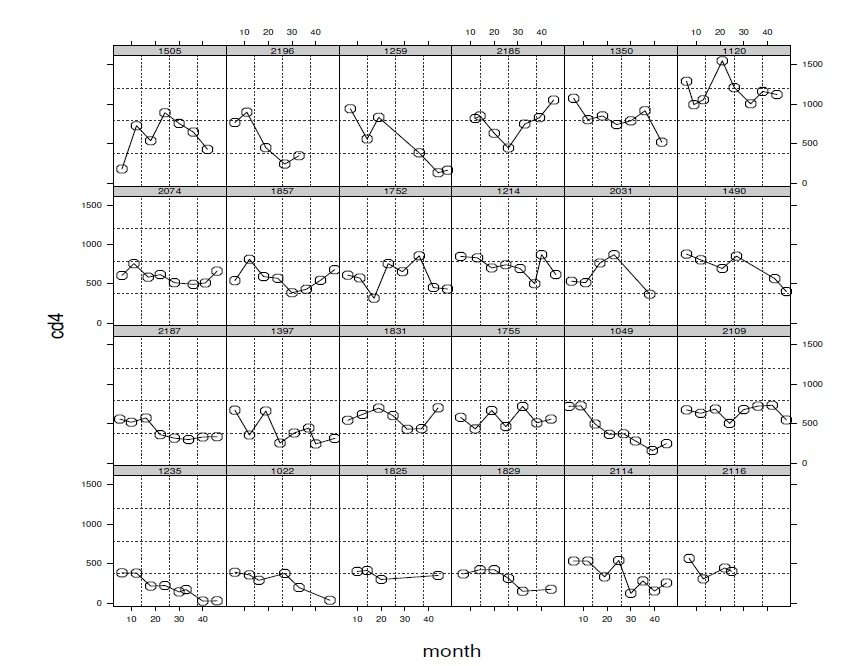
\includegraphics[scale=0.5]{datos.jpg}
	\caption{Una muestra de trayectorias CD4 individuales de los datos del Estudio Multi-Centro de Cohorte contra el SIDA. Belle, G. (2004).}
	\end{figure}
	
	En la situaci\'on com\'un en el que se est\'a interesado en la correlaci\'on de los resultados medidos a factores tales como el grupo de tratamiento o exposici\'on tambi\'en ser\'a \'util para graficar series individuales por el grupo de covarianza. \textit{\citet{belle}}

\subsection{M\'odelos lineales mixtos}

	Muchos m\'odelos estad\'isticos se pueden expresar como m\'odelos que incorporan dos partes: una parte son los efectos fijos, son par\'ametros asociados a toda la poblaci\'on o ciertos niveles de factores experimentales repetibles; otra parte son los efectos al azar, est\'an asociados con los sujetos experimentales o unidades extra\'idas u observados al azar de la poblaci\'on. Los m\'odelos con ambos, tanto el efecto fijo y el efecto al azar se denominan m\'odelos mixtos. \\
	 
	Los m\'odelos mixtos se utilizan principalmente para describir las relaciones entre una dimensi\'on-variable de respuesta final o multidimensional y algunas covariables posiblemente relacionados con los datos observados, agrupandose de acuerdo con uno o m\'as factores de agrupamiento. Tales datos deben incluir datos longitudinales, datos de medidas repetidas.\citet{zhang} 
	 
	 Para un solo nivel de agrupaci\'on de datos correlacionados, los m\'odelos lineales mixtos especifican la $n_{i}-dimensional$ responde al vector $Y_{i}=(Y_{i1},Y_{i2},\cdots ,Y_{inj})^{T}$ para $i=1,2,\cdots,m,$ con un n\'umero total de observaciones $\sum_{i=1}^m n_{i}$ 
	
	\begin{equation}
	 Y_{i}=X_{i}\beta +Z_{i}b_{i}+\epsilon_{i},   i=1,2,\cdots,m,	
	\end{equation}
	
	 \begin{equation}
	 b_{i} \sim N(0,\Psi),    \epsilon_{i} \sim N(0,\delta^{2}\Lambda_{i}),
	 \end{equation}

\noindent
Donde $\beta$ es el vector p-dimensional de efectos fijos \\
los $b_{i}$ son los vectores q-dimensionales de efectos al azar \\
$X_{i}$ son $n_{i} \times p$ matrices regresivas de efectos fijos \\
$Z_{i}$ son $n_{i} \times q$ matrices regresivas de efectos al azar \\
$\epsilon_{i}$ son las $n_{i}-$dimensionales sin un grupo de vectores de errores \\
$\psi$ es una matriz definida sim\'etrica positiva denotando la estructura de la varianza y covarianza entre los efectos al azar \\
$b_{i}$, $\lambda_{i}$ son matrices definidas positivas denotando la estructura de la varianza y la covarianza dependientes sin grupo de errores.\\ 

Los efectos al azar $b_{i}$ y el grupo sin errores $\epsilon_{i}$ se asumen que son independientes para los diferentes grupos y para ser independientes entre s\'i con el mismo grupo. En los modelos lineales mixtos, se supone que la respuesta continua gaussiana es una funci\'on lineal de covariables con coeficientes de regresi\'on que var\'ian sobre los individuos, lo que refleja la heterogeneidad natural debido a factores no medidos. \citet{zhang} 

\subsection{M\'odelos lineales mixtos en el an\'alisis de datos longitudinales}

	En medicina, se utilizan estudios longitudinales para descubrir factores predictivos de enfermedades. Los datos recogidos en un estudio longitudinal son datos longitudinales. En el an\'alisis de datos longitudinales, los modelos lineales mixtos son ampliamente utilizados. Medidas repetidas en datos longitudinales se observan en los sujetos a lo largo del tiempo. Adem\'as de la variable de tiempo, normalmente se observan otras covariables, lo que a su vez requiere una selecci\'on m\'as precisa para buscar el mejor modelo de una gran cantidad de modelos de candidatos. En el an\'alisis de los datos longitudinales por modelos lineales mixtos, la selecci\'on del modelo tambi\'en implica la selecci\'on de covariables y la variaci\'on de la selecci\'on de la estructura de covarianza de los efectos aleatorios y los errores dentro del grupo.\\
	
	En la figura 2.2. Toma una muestra y traza l\'ineas para cada sujeto estratificado por el nivel de carga viral de referencia. Esta cifra sugiere que la mayor carga viral del grupo tiene el menor recuento de $T^{+}CD4$, y sugiere que la variaci\'on entre las mediciones tambi\'en pueden ser menores para el grupo de carga viral basal, en comparación con los grupos medio y bajo. La figura 2.2 tambi\'en se puede usar para identificar las personas que exhiben tendencias temporales que difieren notablemente de otras personas. En el grupo de alta carga viral hay un individuo que parece mejorar dram\'aticamente con el tiempo, y hay una sola medici\'on inusual, donde el recuento de $T^{+}CD4$ es superior a 2000. El trazado de series individuales es un preludio exploratorio a un an\'alisis estad\'istico confirmatorio m\'as cuidadoso.
	
	\begin{figure}[H]
	\centering
	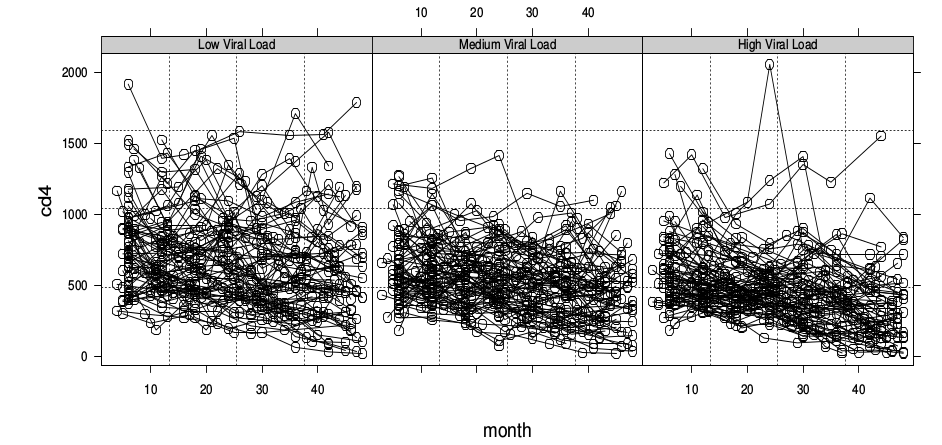
\includegraphics[scale=0.4]{mixed.png}
	\caption{Las trayectorias $T^{+}CD4$ individuales de los datos de la carga viral. Belle, G. (2004).}
	\end{figure}
	
\subsection{VIH}

	El virus de la inmunodeficiencia humana es un retrovirus o virus de \'acido ribonucleico (ARN), la conversi\'on de ARN en \'acido desoxirribonucleico (ADN) es la caracter\'istica definitoria del virus, la cual se lleva a cabo mediante la acci\'on enzim\'atica de la transcriptasa inversa. \\

	Seg\'un la \citet{oms}, el VIH puede trasmitirse por las relaciones sexuales vaginales, anales u orales con una persona infectada, la trasfusi\'on de sangre. Asimismo, puede trasmitirse de la madre al hijo durante el embarazo, el parto y la lactancia.\\

	La infecci\'on por VIH es silenciosa, porque no muestra ning\'un s\'intoma y suele ser diagnosticado por medio del estudio llamado: ensayo inmunoenzimatico ligado a enzimas (ELISA). \citet{bcs}
	
\subsection{SIDA}
	
	Se denomina as\'i, al cuadro cl\'inico que presenta los estadios m\'as avanzados de la infecci\'on por VIH, es decir; se considera cuando la cuenta de linfocitos $T^{+}CD4$ se encuentra por debajo de las 200 c\'elulas en un mililitro o cuando presenta el cuadro complejo de combinaci\'on de coinfecciones relacionadas con el VIH. \citet{bcs}	

\subsection{Relaci\'on VIH - $\mathrm{T^{+}CD4 - T^{+}CD8}$}

	Dos pruebas se pueden utilizar para monitorear el avance del VIH, son los recuentos de las c\'elulas $T^{+}CD4$ y las pruebas de carga viral. Los recuentos de $T^{+}CD4$ indican el estado del sistema inmunitario. Las pruebas de carga viral indican que tan activo est\'a el VIH. Al comienzo estas pruebas deben hacerse con 2 a 4 semanas de diferencia para establecer el “punto de partida” (baseline). Luego deben repetirse aproximadamente cada 3 meses. Las pruebas de carga viral, los recuentos de $T^{+}CD4$, proveer\'a una imagen m\'as clara sobre el riesgo que la enfermedad avance, el estado del sistema inmunitario y la capacidad del organismo para combatir el VIH.\\

	Normalmente, las pruebas sobre el recuento de los varios tipos de gl\'obulos blancos. Un tipo de gl\'obulos blancos son las c\'elulas B, las cuales est\'an involucradas en la producci\'on de anticuerpos. Las c\'elulas B tambi\'en se enfrentan a las infecciones que est\'an por fuera de las c\'elulas. Otro tipo de gl\'obulos blancos son las c\'elulas $T^{+}CD8$, las cuales se enfrentan a las infecciones por dentro de las c\'elulas. El tercer tipo de gl\'obulos blancos son las c\'elulas $T^{+}CD4$, las cuales ayudan a las c\'elulas B y $T^{+}CD8$ a llevar a cabo su labor. Estos gl\'obulos blancos se denominan linfocitos. \\ 

	En las personas VIH negativas, los recuentos normales de $T^{+}CD4$ fluct\'uan entre 600 y 1,500/$mm^{3}$. El recuento normal de $T^{+}CD8$ es de 300 a 800/$mm^{3}$. En general, una persona VIH negativa tiene 2 c\'elulas $T^{+}CD4$ por cada c\'elula $T^{+}CD8$ en la sangre. Sin embargo, en la enfermedad del VIH, el virus normalmente ocasiona una lenta disminuci\'on progresiva de las c\'elulas $T^{+}CD4$, y entre los que no est\'an en terapia para el VIH es com\'un ver invertida la relaci\'on entre $T^{+}CD4$ y $T^{+}CD8$. \\

	Los recuentos normales de $T^{+}CD4$ en las personas con VIH son de 350 a 800. Adem\'as de observar estos recuentos de c\'elulas, es tambi\'en \'util observar los porcentajes relativos de c\'elulas $T^{+}CD4$ y $T^{+}CD8$. El porcentaje de $T^{+}CD4$ es el porcentaje de c\'elulas $T^{+}CD4$ del total del recuento de gl\'obulos blancos. El rango normal es del 28 al 58\%. Un porcentaje de $T^{+}CD4$ por debajo del 14\% indica un diagn\'ostico de SIDA. \citet{ramduth} 
	
\subsection{Clasificaci\'on establecida de la infecci\'on por el VIH y enfermedades relacionadas}

	Seg\'un la Organizaci\'on Mundial de la Salud, en 1990 se desarroll\'o un sistema de estadificaci\'on cl\'inica de 4 estadios a efectos cl\'inicos que solo est\'a basado en adultos. Las clasificaciones cl\'inicas de los centros para el control y la prevenci\'on de enfermedades de los Estados Unidos y de la OMS, reconocen la infecci\'on primaria por el VIH, tambi\'en proponen la aparici\'on de eventos nuevos o recurrentes de estatificaci\'on cl\'inica y la clasificaci\'on inmunol\'ogica, sean usados para evaluar a los individuos cuando ya est\'an recibiendo antirretrovirales. \citet{oms} 

\subsection{Clasificaci\'on cl\'inica de la infecci\'on establecida por el VIH }

	Los eventos cl\'inicos, se aplican para clasificar la enfermedad por el VIH en adultos afectados por el VIH se dividen en aquellos donde pueda hacerse un diagn\'ostico cl\'inico presuntivo y aquellos que requieren un diagn\'ostico definitivo. En la Tabla se muestra el estadio cl\'inico con su relaci\'on en t\'erminos simplificados para describir la variedad de s\'intomas relacionados con la infecci\'on por el VIH: asintom\'atico, s\'intomas leves, s\'intomas avanzados y s\'intomas graves. La Tabla resume los eventos de estadificaci\'on cl\'inica. \citet{oms} 
	
\begin{table}[H]	
\begin{center}
\begin{tabular}{|l|l|}
\hline
S\'intomas asociados a la infecci\'on por el VIH & Estadio Cl\'inico de la OMS \\ \hline
Asintom\'atico & 1  \\ \hline
S\'intomas leves & 2  \\ \hline
S\'intomas avanzados & 3  \\ \hline
S\'intomas graves & 4  \\ \hline

\end{tabular}
\caption{Clasificaci\'on Cl\'inica  de la OMS de la infecci\'on por el VIH establecida. OMS (2009).}
\label{tabla:estadios}
\end{center}
\end{table}

\subsection{Clasificaci\'on inmunol\'ogica para la infecci\'on establecida por el VIH}

	Seg\'un sea la clasificaci\'on definida por el estado cl\'inico o por el estado inmunitario, el paciente siempre requiere tratamiento antirretroviral, especialmente cuando la enfermedad es avanzada desde el punto de vista cl\'inico, pero a veces puede retrasarse el inicio del tratamiento, si el estado inmunitario indica que solo hay una inmunodeficiencia leve o insignificante y el paciente esta asintom\'atico o solo tiene s\'intomas leves. \citet{oms} 
	
\begin{table}[H]	
\begin{center}
\begin{tabular}{|l|l|l|l|l|}
\hline
\multicolumn{5}{|c|}{Valores de $T^{+}CD4$ relacionados con la edad} \\ \hline 
Inmunodeficiencia asociada al VIH & $\leq 11$ meses & 12-35 meses & 36-59 meses & $\geq 5$ a\~nos \\ \hline
Ninguna & $>35$ & $>30$ & $>25$ & $>500$ \\ \hline 
Leve & 30-35 & 25-30 & 20-25 & 350-499 \\ \hline
Avanzada & 25-29 & 20-24 & 15-19 & 200-349 \\ \hline
Grave & $<25$ & $<20$ & $<15$ & $<200mm^{3}$ \\ \hline

\end{tabular}
\caption{Clasificaci\'on inmunol\'ogica propuesta por la OMS para la infecci\'on establecida por el VIH. OMS (2009).}
\label{tabla:inmunologica}
\end{center}
\end{table}

\subsection{VIH en Venezuela}

	En Venezuela se estima que la epidemia de VIH es concentrada, las personas que viven con el virus son aproximadamente 101.871, de las cuales 64\% corresponde al sexo masculino, pero se ha evidenciado no poseer mucha data correspondiente a la epidemia, solo se muestran casos muy antiguos y no se ha actualizado la informaci\'on, los reportes avalados por el gobierno, no poseen informaci\'on seria y confiable, no se dispone de mucha m\'as informaci\'on, solo la obtenida en 2012 sobre las caracter\'isticas generales de la epidemia. \citet{narrative} \\
	
	En la siguiente tabla se muestra la mortalidad en Venezuela desde el periodo 2007-2011, haciendo referencia que la tasa de mortalidad espec\'ifica por cada 100 mil habitantes por causa para VIH/SIDA, aument\'o y se increment\'o en ambos sexos.
	
\begin{table}[H]	
\begin{center}
\begin{tabular}{|l|l|l|l|l|l|l|}
\hline
A\~no & Hombres & Tasa & Mujeres & Tasa & Total & Tasa  \\ \hline
2007 & 1288 & 9.34 & 382 & 2.79 & 1670 & 6.08 \\ \hline
2008 & 1223 & 8.73 & 409 & 2.94 & 1632 & 5.84 \\ \hline
2009 & 1327 & 9.32 & 408 & 2.88 & 1735 & 6.11 \\ \hline
2010 & 1380 & 9.55 & 450 & 3.13 & 1830 & 6.35 \\ \hline
2011 & 1612 & 10.99 & 554 & 3.79 & 2166 & 7.40 \\ \hline

     
\end{tabular}
\caption{Mortalidad por VIH/SIDA seg\'un a\~no y sexo. Venezuela. 2002-2011. Rep\'ublica Bolivariana de Venezuela (2014).}
\label{tabla:mortalidad}
\end{center}
\end{table}

	Sigue siendo una aspiraci\'on de los diversos actores involucrados en la prevenci\'on y control de la enfermedad y una prioridad para la comunidad nacional, poder disponer de la estimaci\'on y proyecci\'on de la situaci\'on epidemiol\'ogica del VIH/SIDA actualizada, paso indispensable para poder cumplir la Meta 7 de los Objetivos del Milenio de las Naciones Unidas: Haber detenido y empezado a revertir la incidencia del VIH-SIDA en el año 2015.  La mortalidad por VIH/SIDA, se caracteriz\'o por un aumento progresivo. La tendencia en el lapso de 21 a\~nos es al ascenso. \textit{\citet{alerta}} \\

	Las fallas y deficiencias identificadas en los sistemas de vigilancia epidemiol\'ogica de los casos de VIH/SIDA, no permiten identificar oportunamente los cambios recientes en las tendencias de infecci\'on por el VIH, debido entre otras razones, al largo per\'iodo de latencia de la enfermedad. La introducci\'on de tratamientos antirretrovirales ha contribuido sustancialmente a la sobrevida de los pacientes.\\

	Tomando a Venezuela como un todo, algunos estudios demuestran la alarmante situaci\'on del VIH en el pa\'is. En particular, porque no se dispone de mucha informaci\'on oficial y ver\'idica, permitiendo aclarar la situaci\'on, en este caso solo se toma en cuenta el caso particular del estado M\'erida, haciendo \'enfasis en su geograf\'ia por municipios, para poder estudiar mejor los cambios que ha devenido en el tiempo.

\begin{figure}[H]
	 \centering
	 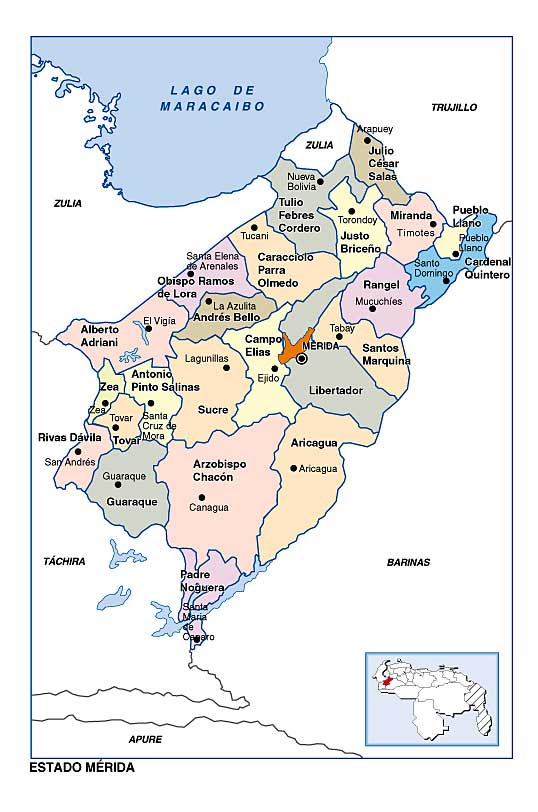
\includegraphics[scale=0.5]{merida.jpg}
	 \caption{Mapa del Estado M\'erida con sus municipios. Alcaldia del Estado M\'erida (2016)}
	 \end{figure}

\subsection{Lenguaje R para el computo estad\'istico}

El entorno de programaci\'on R es un clon de los lenguajes S y S-plus, de tal forma que muchos programas escritos en S y S-plus pueden ejecutarse en R sin modificaciones. S y S-plus son lenguajes de muy alto nivel diseñados para: La exploraci\'on y visualizaci\'on de datos; el modelado estad\'istico; y la programaci\'on con datos. \\

R es un entorno de programaci\'on para el an\'alisis estad\'istico y gr\'afico de datos, que cada vez se hace m\'as popular entre los investigadores de todas las disciplinas. Tiene muchas ventajas y es oportuno y pertinente para los investigadores de cualquier \'area del saber. \\

Como software libre es aprobado por varios motivos: trasmite valores socialmente positivos (libertad individual, conocimiento compartido, solidaridad y cooperaci\'on); se aproxima al m\'etodo cient\'ifico, porque permite el examen y mejora del c\'odigo desarrollado por otros ususarios y la reproducibilidad de los resultados obtenidos; pueden adquirirse de manera legal y gratuita copias del programa, sin necesidad de licencias personales o acad\'emicas. \\

Aparte de su faceta de software libre, R tiene algunas ventajas espec\'ificas: por ejemplo, su sintaxis b\'asica es sencilla e intuitiva, lo que se traduce en un aprendizaje r\'apido y c\'omodo; adem\'as, tiene una enorme comunidad de usuarios, estructurada alrededor de la \textit{Comprensive R Archive Network}, CRAN,lo que desarrolla cada d\'ia nuevos paquetes que extienden sus funcionalidades y cubren casi todas las necesidades computacionales y estad\'isticas de un cient\'ifico.

\subsection{Adquisici\'on y licencia}

El entorno R es un software libre en c\'odigo fuente bajo la definici\'on dada en la licencia GNU (General PublicLicense) de la FSF (Free software fundation), el cual puede ser descargado ya sea como c\'odigo fuente o como un ejecutable para los sistemas operativos Linux, Windows o MacOS.

\subsection{Interfaz de usuario}

La interacci\'on con el usuario se basa en una interfaz de usuario llamada RStudio, ambiente de desarrollo integrado que permite una interacci\'on r\'apida y amigable con R, adem\'as del desarrollo de c\'odigo de forma interactiva.

\begin{figure}[H]
\centering
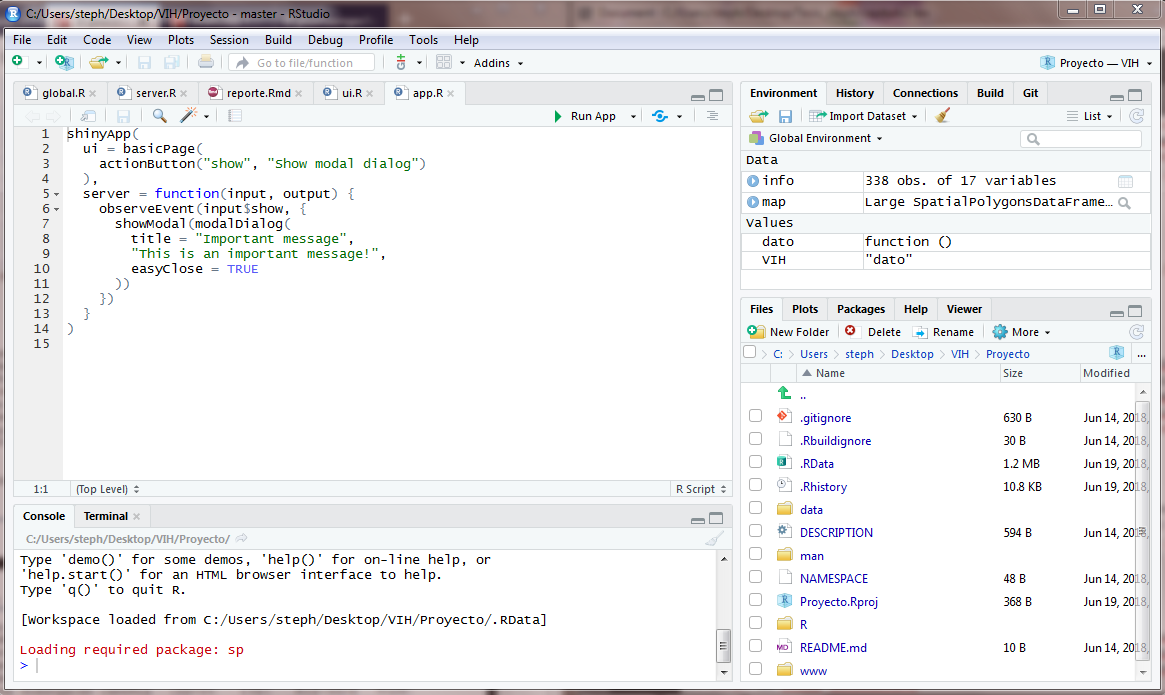
\includegraphics[scale=0.4]{RStudio.PNG}
\caption{Interfaz de RStudio (Versi\'on 1.1.453)}
\end{figure}

\subsection{Lenguaje de programaci\'on}

En su gram\'atica, la sintaxis del lenguaje R es similar a la de C y C++, pero su sem\'antica sigue los paradigmas de la programaci\'on funcional y la programaci\'on orientada a objetos, lo que implica que el lenguaje tiene la capacidad de manipular directamente los objectos del lenguaje, aplicar reglas de sustituci\'on y evaluar expresiones. \citet{grun}

R es un lenguaje orientado a objetos, tal que, inclusive los tipos m\'as b\'asicos de datos, tales como: booleanos, enteros, reales, caracteres, vectores, matrices, listas y hojas de datos son objetos mismos. Esta caracter\'istica permite que el usuario interact\'ue de forma transparente, ya que las llamadas se realizan a funciones gen\'ericas, como print, summary o plot, las cuales determinan internamente que m\'etodo debe ser llamado dependiendo de la clase de objetos a las que pertenecen sus argumentos. \\

R soporta internamente dos implementaciones para la programaci\'on orientada a objetos llamadas S3, que fue diseñado para uso interactivo, y S4, el cual supera las deficiencias de S3, y adiciona nuevos elementos. Adicionalmente, el usuario puede definir sus propias clases y los m\'etodos asociados a ellas.\\

\subsection{Shiny}

Shiny es un paquete R que facilita la creaci\'on de aplicaciones web interactivas (aplicaciones) directamente desde R. Las aplicaciones Shiny est\'an contenidas en un solo script llamado app.R. La secuencia de comandos app.R ubicado en un directorio (por ejemplo, nuevo/) y la aplicaci\'on se puede ejecutar con runApp ("nuevo").\\

app.R tiene tres componentes:

   \begin{itemize}
     \item un objeto de interfaz de usuario
     \item una funci\'on de servidor
     \item una llamada a la funci\'on shinyApp
     \end{itemize}

El objeto de la interfaz de usuario (ui) controla el diseño y la apariencia de la aplicaci\'on. La funci\'on del servidor contiene las instrucciones que la computadora necesita para construir la aplicaci\'on. Finalmente, la funci\'on shinyApp crea objetos de la aplicación Shiny desde un par de UI / servidor expl\'icito.

\begin{figure}[H]
\centering
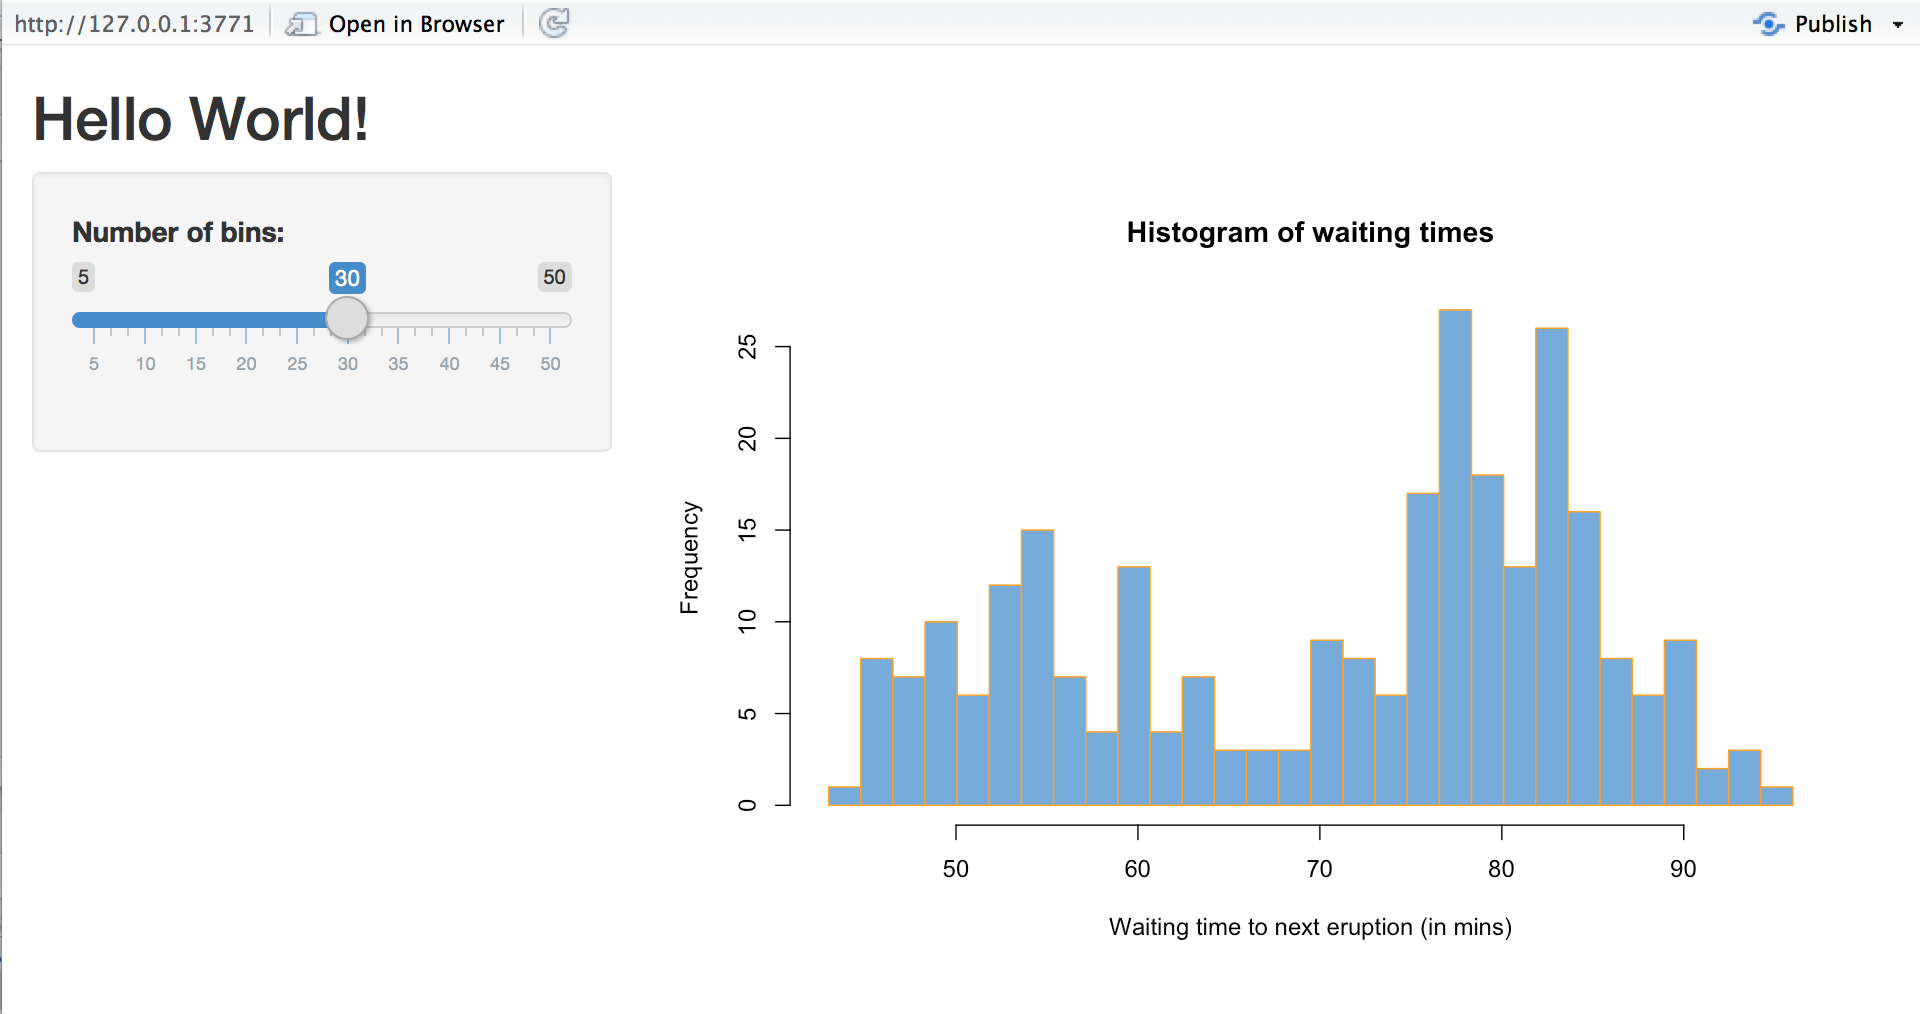
\includegraphics[scale=0.5]{shiny.png}
\caption{Aplicaci\'on en Shiny}
\end{figure}

\chapter{Fundamentos metodol\'ogicos}

	Se plante\'o la estructura a seguir por el trabajo, detallando el enfoque, tipo, nivel, dise\~no de la investigaci\'on y la metodolog\'ia implementada entre otros, el cual fue de vital importancia para el desarrollo de la misma. 
	
\section{Enfoque de la investigaci\'on}
	
	La investigaci\'on se desarrollo siguiendo un enfoque cuantitativo, como lo indican  \citet{pallela}, “la investigaci\'on cuantitativa requiere el uso de instrumentos de medici\'on y comparaci\'on, proporcionando datos cuyo estudio necesita la aplicaci\'on de m\'odelos matem\'aticos y estad\'isticos, el conocimiento est\'a basado en hechos”.  

\section{Tipo o nivel de investigaci\'on}
	
	Este proyecto plante\'o un tipo de investigaci\'on de campo, seg\'un como lo indican \citet{pallela},  la investigaci\'on de campo “consiste en la recolecci\'on directamente de la realidad donde ocurren los hechos, sin manipular o controlar variables” ya que permite indagar los efectos de la interrelaci\'on entre los diferentes tipos de variable en lugar de los hechos.\\

	En este punto se debe determinar la profundidad que abarca esta investigaci\'on, teniendo en cuenta que de acuerdo con \citet{arias} el nivel de la investigaci\'on es definido como “grado de profundidad con que se aborda un fen\'omeno u objeto de estudio”\\

	En este sentido, se tiene que dadas las caracter\'isticas del proyecto, se asocia con un nivel descriptivo, tal como lo indican \citet{pallela},  “hace \'enfasis sobre conclusiones dominantes o sobre como una persona, grupo o cosa se conduce o funciona en el presente” esto debido a que se medir\'an los datos extra\'idos sin alterarlos para ser mostrados en el sistema.\\

	Cuando se habla de un nivel descriptivo junto con una investigaci\'on de tipo de campo, en ella no se formulan hip\'otesis y las variables se enuncian en los objetivos de la investigaci\'on desarrollada.
	
\section{Dise\~no de investigaci\'on}
	
	Seg\'un \citet{arias}, el dise\~no de la investigaci\'on es “la estrategia general que adopta el investigador para responder al problema planteado”  puesto es vital establecer una correcta secuencia de pasos para elaborar el prototipo de  \textit{software}  dando soluci\'on a la problem\'atica principal de la investigaci\'on. \\
	
	Con este enfoque, es evidente entonces, el trabajo segui\'o un dise\~no no experimental para datos longitudinales retrospectivos, enfocado en el uso de informaci\'on existente, de acuerdo con lo dicho por  \citet{pallela} al definir el dise\~no no experimental como:

\begin{quote}
Es el que se realiza sin manipular en forma deliberada ninguna variable. El investigador no sustituye intencionalmente las variables independientes. Se observan los hechos tal y como se presentan en su contexto real y en un tiempo determinado o no, para luego analizarlos. Por lo tanto, este dise\~no no se construye una situaci\'on espec\'ifica sino que se observan las que existen. Las variables independientes ya han ocurrido y no pueden ser manipuladas, lo que impide influir sobre ellas para modificarlas. 
\end{quote}

	Esto indica que no hubo manipulaci\'on de variables. Esta investigaci\'on presenta una modalidad de proyecto especial que, como lo indican \citet{pallela}, los proyectos especiales “destinados a la creaci\'on de productos que puedan solucionar deficiencias evidenciadas, se caracterizan por su valor innovador y aporte significativo”, ya que se crear\'a un \textit{software} aplicable al \'area de estudio.

\section{Poblaci\'on y muestra}

Seg\'un \citet{morles} la poblaci\'on o universo al conjunto para el cual fueron validas las conclusiones que se obtuvieron de los elementos o las unidades (personas, instituciones o cosas) involucradas en la investigaci\'on.\\

En este sentido, se tiene que para las fases de elaboraci\'on y pruebas del prototipo de \textit{software}, se plante\'o utilizar archivos con extesi\'on .csv, como formato de datos de entrada a la aplicaci\'on.\\

La informaci\'on para los archivos de prueba proviene de vistas minables de la base de datos de tipo relacional, desarrollada en \textit{PostgreSQL} del Laboratorio de Investigaciones Hormonales del Instituto Aut\'onomo Hospital Universitario de los Andes, que alberga al programa para pacientes con VIH, que cuenta con una poblaci\'on registrada de 45.649\\

Esta informaci\'on fue  filtrada, par considerando los siguientes criterios:\\
\begin{itemize}
    \item La base de datos del Laboratorio de Investigaciones Hormonales IAHULA, no s\'olo almacena informaci\'on del Programa de Pacientes con VIH, las vistas minables estan conformadas por pacientes confirmados por las pruebas \textit{Elisa} y {Western Blot} para VIH
    \item En las vistas minables para  las pruebas s\'olo se categorizar\'an pacientes con residencia en el Estado Mérida
    \item Las vistas minables s\'olo las integraran pacientes con m\'as de tres años en seguimiento. Dado que los modelos son para datos longitudinales.
    \item Se categorizaron los pacientes por semestres y en cada lapso en medicados y no medicados.
\end{itemize}

Bajo estas condiciones se generó una vista minable (muestra) con 115 registros de pacientes, con una secci\'on transversal conformada por la edad el g\'enero y el municipio de residencia  y una secci\'on longitudinal con  informaci\'on entre Enero del año 2007 y Diciembre del año 2013. sobre el Log$_{10}$ de la carga viral plasm\'atica y las sub-poblaciones linfocitaria de c\'elulas T$^{+}$ CD4 y  T$^{+}$ CD8.\\

\section{T\'ecnicas e instrumentaci\'on para la recolecci\'on de datos}

En el desarrollo de este prototipo de \textit{software} es de vital importancia contar con una correcta t\'ecnica de recolecci\'on de datos y un instrumento adecuado para dicha t\'ecnica, pues fueron la base para lograr un efectivo an\'alisis estad\'istico, y as\'i como eficaces resultados en la fase de pruebas. Todo esto, teniendo en cuenta que, seg\'un \citet{hurtado} la selecci\'on de t\'ecnicas e instrumentos de recolecci\'on de datos implica determinar por cu\'ales medios o procedimientos el investigador obtendr\'a la informaci\'on necesaria para alcanzar los objetivos de la investigaci\'on.\\

Para efectos de esta investigaci\'on, se tuv\'o que la t\'ecnica de recolecci\'on de datos seleccionada es la observaci\'on no participante, indirecta y estructurada, la cual se ajusta a este de investigaci\'on, ya que como lo indican \citet{pallela} la observaci\'on es indirecta:

\begin{quote}
Cuando el investigador entra en conocimiento del hecho o fen\'omeno a trav\'es de las observaciones realizadas anteriormente por otra persona. Esto \'ultimo ocurre cuando se utilizan libros, revistas, informes, grabaciones, fotograf\'ias, realizadas con lo que se esta investigando, los cuales han sido obtenidos o elaborados por personas que antes se ocuparon de lo mismo.
\end{quote}

Esto debido, a que los datos usados provienen de la data existente del IAHULA, las cuales fueron tomadas previamente por otro investigador, por lo que no se intervino directamente en su recolecci\'on. Para esta fase de la investigaci\'on se realiz\'on una exportaci\'on de las tablas que conforman la base de datos que almacenaban informaci\'on sobre: Paciente, Pruebas, Resultados a archivos de texto plano, luego estos archivos fueron exportados a \textit{Microsoft Oficce Excel}, con formato .cvs donde los registros por pacientes fueron filtrados para conformar muestras an\'onimas y su direcci\'on categorizarla por municipios.
\section{Entorno de trabajo}

\subsection{\textit{Software} de desarrollo}

Para la realizaci\'on del prototipo de \textit{software}, fue necesario definir el entorno de desarrollo usado, se selecciono el lenguaje de programaci\'on R, dado que es un lenguaje de c\'odigo abierto bajo el paradigma de desarrollo colaborativo.  Como  herramienta de desarrollo integrada \textit{Integrated Development Environment, IDE} para lenguaje  R, se seleccion\'o  RStudio, dado su bran abanico de paquetes e integraci\'on con repositorios Git  que permite llevar  un control de versiones del sistema apoyado en el servicio de alojamiento gratuito de GitHub.

\subsection{\textit{Hardware} utilizado}

En la parte de hardware usado, se cuent\'o con dos computadoras (laptop y de PC de escritorio), con las caracter\'isticas descritas en la tabla:

\begin{table}[H]
\begin{center}
\begin{tabular}{|l|l|l|l|}
\hline
Componente & Laptop & PC Escritorio \\ \hline
CPU & Intel Core i3-380 & Intel Core i5-2310 \\ \hline
RAM & 4GB & 4GB \\ \hline
S.O & Windows 7 Ultimate & Windows 10  \\ \hline

\end{tabular}
\caption{Caracter\'isticas de los computadores a usar}
\label{tabla:componente}
\end{center}
\end{table}

\section{Metodolog\'ia}

Para el desarrollo de este trabajo se implement\'o  una metodolog\'ia para el desarrollo del \textit{software} en espiral  la es un m\'odelo del ciclo de vida del \textit{software} donde el esfuerzo del desarrollo es iterativo, tan pronto termina un esfuerzo, ah\'i mismo comienza el otro; adem\'as en cada ejecuci\'on del desarrollo se sigue cuatro pasos principales:

1. Determinar o fijar los objetivos: se definen los objetivos espec\'ificos para posteriormente identificar las limitaciones del proceso y del sistema de \textit{software}; adem\'as se dise\~na una planificaci\'on detallada de gesti\'on y se identifican los riesgos.

2. An\'alisis de riesgo: se efect\'ua un an\'alisis detallado para cada uno de los riesgos identificados del proyecto, definiendo los pasos a seguir para reducir los riesgos y luego analizarlos para planear las estrategias alternativas.

3. Desarrollar, verificar y validar: despu\'es de realizar el an\'alisis de riesgo, se elige un paradigma para el desarrollo del sistema de \textit{software} y se desarrolla.

4. Planificar: el proyecto se revisa, del cual se toma la decisi\'on si se debe continuar con un ciclo posterior al de la espiral. Si se decide continuar, se desarrollan los planes para la siguiente fase del proyecto. \citet{spiral}

\begin{figure}[H]
\centering
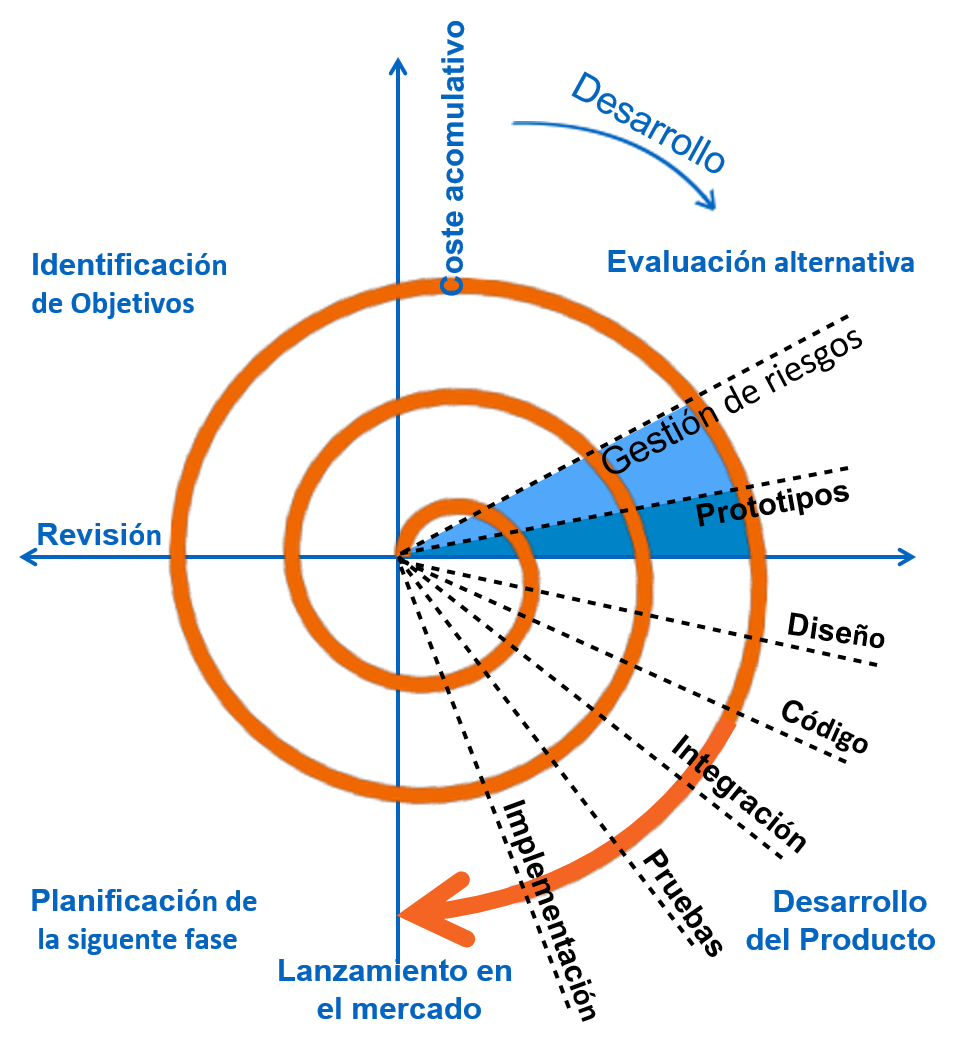
\includegraphics[scale=0.5]{espiral.jpg}
\caption{Modelo espiral del proceso de \textit{software} Boehm B. (1988).}
\end{figure}

Los nuevos requerimientos del sistema se definieron con todos los detalles posibles, esto implica generalmente el entrevistarse con un n\'umero determinado  de usuarios que representar\'an a todos los usuarios tanto externos como internos y otros aspectos del sistema existente. Un prototipo preliminar se cre\'o  para el desarrollo del nuevo \textit{software}  partiendo de un diseño hecho del sistema que se construy\'o del prototipo inicial. Esto es generalmente un sistema  scaled-down, y represent\'o una aproximaci\'on de las caracter\'isticas del producto final.\\
 
Este primer prototipo se desarrollo bajo las siguientes caracter\'isticas u objetivos de \textit{software} a alcanzar:  las funciones base para la carga de datos, los c\'alculos para el ajuste de modelos para los datos longitudinales y el desarrollo de los gr\'aficos se realizar\'ia bajo los paquetes que proporciona lenguaje R en su CRAN y en sus extensiones; la interfaz gr\'afica de usuario (GUI)  ser\'ia bajo un ambiente WEB simple y ligera, que se adaptara a la GUI del Laboratorio de Investigaciones Hormonales del IHULA, donde el gasto computacional fuera la estimaci\'on del modelo para datos longitudinales, esta se realizar\'ia en el lenguaje Java y se emplear\'ian el  paquete rJava para la conexi\'on lenguaje R y Java, adem\'as de JDK (\textit{Java SE Development Kit}) Eclipse. Durante esta etapa el an\'alisis de riesgo determin\'o que al desarrollar la GUI de usuarios bajo Java, seria necesario tener a la disposici\'on un servidor de forma permanente, lo que hace que la aplicaci\'on fuera poco portable. As\'i que se toma la desici\'on de cambiar el ambiente de desarrollo para la GUI.\\ 

Un segundo diseño de \textit{software} fue desarrollado por un procedimiento cu\'adruple: Evaluaci\'on del primer prototipo en t\'erminos de sus fuerzas, debilidades, y riesgos; Definir los requisitos del segundo prototipo; Planeando y desarrollando el segundo prototipo; Construyendo y probando el segundo prototipo. \\

El segundo diseño de \textit{software} mantuvo las caracter\'isticas seleccionadas para el primer diseño sobre el c\'alculos y las herramientas gr\'aficas pero la GUI se desarrolla empleando el paquete \textit{Shiny} del IDE RStudio, lo que permite tener un servidor local para cada usuario. \\

Adem\'as, se construy\'o el sistema final al que se denomin\'o HIVmlm (Human Immunology Virus linear model mixed effects), basado en el segundo diseño pero mejorando las caracter\'isticas de la GUI en la  Figura 3.3, se  muestra el\textit{wireframe} siguiendo el modelo basado en experiencia de usuario. El sistema final se eval\'uo y se probo con metodos de caja blanca y caja negra.\\


\begin{figure}[H]
\centering
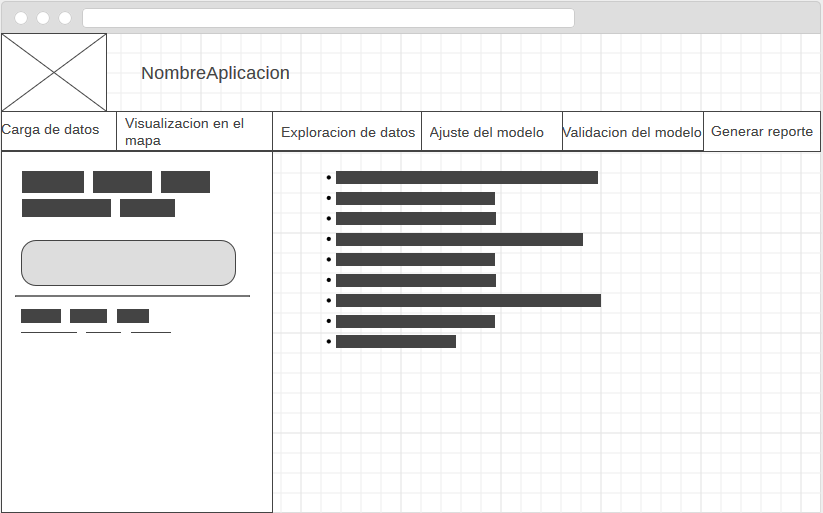
\includegraphics[scale=0.6]{etapa1_wireframe.png}
\caption{Wireframe base de la interfaz gr\'afica de usuario}
\end{figure}






\chapter{Desarrollo de la investigaci\'on}

Este cap\'itulo comprende la exposici\'on detallada del desarrollo de versi\'on final del \textit{software}  siguiendo una metodolog\'ia en espiral; se describe las diferentes iteraciones del ciclo y las fases de la elaboraci\'on del \textit{software} al que se denomin\'o HIVmlm (Human Immunology Virus linear model mixed effects).\\

\section{Desarrollo}

Siguiendo la metodolog\'ia de trabajo en espiral, se construy\'o  una lista de los m\'odulos a desarrollar en la aplicaci\'on acorde a los objetivos planteados en la investigaci\'on, y siguiendo los paradigmas para el desarrollo de paquetes en lenguaje R, presentados por \citet{test} y por el creador del paquete \emph{formatR} \citet{format}. Los m\'odulos desarrollados fueron:


\begin{enumerate}
\item Carga de datos
\item Exploraci\'on de los datos
\item Visualizaci\'on en el mapa
\item Ajuste del m\'odelo
\item Validaci\'on del m\'odelo
\item Generar reporte
\end{enumerate}
   
 Cada m\'odulo paso por las etapas del m\'odelo en espiral, en este caso, 4 etapas planificadas, estas etapas se realizaron dentro del tiempo establecido, con una revision semanal por parte de la tutora, dichas etapas se detallar\'an a continuaci\'on:

\section{Etapa 1}

Siguiendo cada una de las etapas de la metodologóa en espiral el desarrollo de \textit{software}, se comienza por el an\'alisis de riesgo y el dise\~no de prototipos. Para el desarrollo de la aplicaci\'on se seleccion\'o Lenguaje R. \\

Los m\'etodos para el dise\~no de las funciones primarias en R ser\'an los diagramas de flujo; y para su codificaci\'on se seguir\'an las normas de estilo para codificaci\'on en R, sugeridas por \citet{test} y por el creador del paquete \emph{formatR} \citet{format}, adem\'as se establecer\'an la dependencia con las funciones de c\'odigo base y las recomendadas para desarrollo en R.\\

Se desarroll\'o el m\'odulo de Carga de Datos  asociados a los  pacientes, primero se filtr\'o la informaci\'on para el caso de estudio, la cual  pertenece a  la Base de Datos original del Laboratorio de Investigaciones Hormonales del Instituto Aut\'onomo Hospital Universitario de Los Andes, esto con el objetivo de dar cumplimiento a las Leyes de protección para personas con VIH en Venezuela y las recomendadas por las Organizacion Panamericana (PAHO) y Mundial de la Salud (OMS),  obtiendo informaci\'on relevante para su  representaci\'on en la aplicaci\'on y careciendo de forma absoluta de información de tipo personal o familiar.\\

Se procedi\'o a desarrollar el analisis de riesgos, que incluye, en este caso,  determinar las herramientas usadas para construir el prototipo de \textit{software}, se utiliz\'o para la elaboraci\'on del prototipo, el lenguaje de programaci\'on R y la herramienta \textit{RStudio}, que es un entorno de desarrollo integrado (IDE) para el lenguaje R, dedicado al estudio de la computaci\'on estad\'istica y gr\'afica,  tambi\'en se utilizo el paquete de R, \textit{Shiny}.\\

El desarrollo del prototipo de \textit{software} HIVmlm (Human Immunology Virus linear model mixed effects) parti\'o de la lista de m\'odulos antes expuestos.

\section{Etapa 2}

En la etapa 2, se decidi\'o realizar, la creaci\'on del paquete desde \textit{RStudio}, y as\'i realizar la estructura que debe tener el paquete, adaptandose a \textit{Shiny}. La creaci\'on del paquete de R, dadas sus ventajas siendo una de las principales, permitir probar el paquete sobre varias plataformas distintas (Linux, Mac y Windows) autom\'aticamente, el c\'odigo est\'a p\'ublicamente disponible en la cuenta \textit{GitHub}. \\

\subsubsection{Estructura del paquete}

La estructura es generada por package.skeleton, y sigue la siguiente: los archivos NAMESPACE y DESCRIPTION, y los directorios R y data, todo esto para mantener una colecci\'on coherente del c\'odigo.

\subsubsection{Archivo DESCRIPTION}

El archivo DESCRIPTION contiene la siguiente informaci\'on b\'asica:

\begin{figure}[H]
\centering
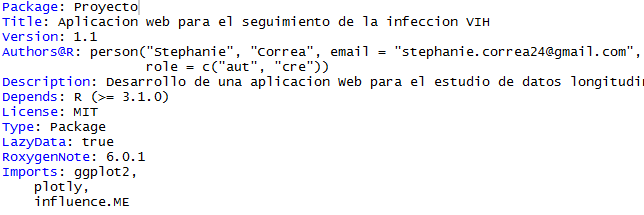
\includegraphics[scale=1]{description.PNG}
\caption{Configuraci\'on b\'asica de la aplicaci\'on }
\end{figure}

\subsubsection{Archivo NAMESPACE}

El archivo NAMESPACE lo crea RStudio, en base al archivo DESCRIPTION previamente creado, es de vital importancia este archivo, porque representa la autenticidad del paquete ante otros paquetes. Se genera al utilizar la siguiente expresi\'on:

\begin{figure}[H]
 \centering
 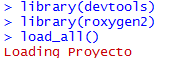
\includegraphics[scale=1]{creacion.png}
 \caption{Creaci\'on de los manuales del paquete}
 \end{figure}
  
 Se realizaron 3 archivos .R:

\begin{itemize}
\item global.R
\item ui.R
\item server.R
\end{itemize}

Por \'ultimo, se realiz\'o el reporte que debe seguir la extensi\'on .Rmd, siguendo la metodologu\'ia del paquete Knitr, paquete que ayuda a la implementaci\'on del reporte en varios formatos. \\

El archivo global.R contiene todas las librerias asociadas para que funcione la aplicaci\'on, y la carga de los archivos asociados a la carga y visualizaci\'on del mapa.\\

El archivo ui.R contiene la estructura gr\'afica que muestra la aplicaci\'on, con los m\'odulos antes expuestos, se procedi\'o a crear la estructura b\'asica, con el diseño planteado por el wireframe, basado en la experiencia de usuario; conteniendo una estructura sencilla y funcional.\\

El archivo server.R contiene todos los c\'alculos y analisis estad\'istico, relativos a la aplicaci\'on, cada m\'odulo realizado en el archivo ui.R tiene una funci\'on relacionada, con la elaboraci\'on y construcci\'on de cada m\'odulo. server.R contiene una funci\'on que recibe todas la entradas y salidas relativas del archivo ui.R. \\

Se realiz\'o el plan de desarrollo para realizar la codificaci\'on de la aplicaci\'on.   

\section{Etapa 3}

Se desarrollo la construcci\'on de los archivos antes mencionados, con la elaboraci\'on de las funciones pertinentes para elaborar los diferentes modulos.

\subsection{Manejo de versiones}
Se desarroll\'o el  \textit{software} en \textit{RStudio}, y se procedi\'o a realizar un control de versiones de la aplicaci\'on por medio de las herramientas  \textit{Git} y  \textit{GitHub}, lo que permiti\'o un mejor manejo de lo realizado en cada etapa de la investigaci\'on.

\begin{figure}[H]
\centering
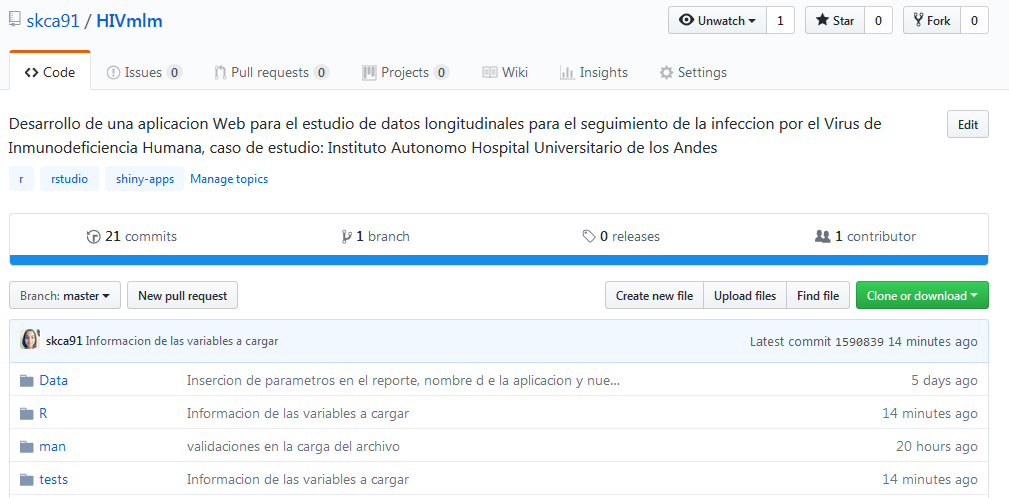
\includegraphics[scale=0.6]{github.png}
\caption{Cuenta alojada de GitHub de la aplicaci\'on}
\end{figure}


\subsection{Filtrado de los datos}

Se ha trabajado con datos recogidos por el Instituto Aut\'onomo Hospital Universitario de los Andes del estado M\'erida, desde el per\'iodo 2007-1 hasta el 2013-2. Los datos registrados, en el per\'iodo de estudio, son 1610. Los casos de VIH se han asignado a partir de la fecha de inicio del tratamiento, y en caso de no saberse, por la fecha de declaraci\'on. Se ha agregado la incidencia cada 6 meses (semestres), formando as\'i dos series temporales por año.\\

Antes del filtrado de la informaci\'on, se usaron datos de prueba para los diferentes pruebas con respecto a la carga del archivo, para esta carga se necesitaba un archivo con extension .csv, con cabecera bien definida dentro del archivo y los nombres de las variables que se necesitaban para la implementaci\'on, se conto con un archivo de extension .R, archivo usado para la creaci\'on del archivo .csv, una vez obtenido el archivo, se procedio a la carga de la informaci\'on en la aplicaci\'on.
\\

Una de las limitaciones en la carga de los archivos es la extensi\'on, solo acepta extensi\'on .csv, siguiendo unas reglas definidas, con respecto a los nombres de las variables.
\\

En esta etapa se logr\'o la elaboraci\'on del m\'odulo de la carga de datos, luego de realizar varias pruebas, en este caso, se logr\'o el prototipo 1 y los objetivos planteados para este prototipo, logrando as\'i planificar la nueva etapa.
\\

\begin{figure}[H]
\centering
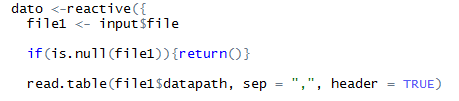
\includegraphics[scale=0.8]{archivo2.PNG}
\caption{Implementaci\'on en R de la carga de archivo}
\end{figure}

Para el desarrollo del m\'odulo de Exploraci\'on de datos, se usaron las librer\'ias de R, plotly y ggplot2.\\

\subsection{Exploraci\'on de datos}

Este m\'odulo esta compuesto por 3 secciones, que comprende el g\'enero, la edad y las cargas con respecto a la carga viral plasm\'atica, las c\'elulas $T^{+}CD4$ y c\'elulas $T^{+}CD8$; para la elaboraci\'on de la categor\'ia por g\'enero, primero se filtraron los datos por per\'iodos, tenemos los per\'iodos de 20071 hasta 20132, cada per\'iodo esta comprendido por semestres, es decir, un año esta compuesto por dos per\'iodos, en este caso, se filtr\'o la informaci\'on, para omitir los datos faltantes con respecto a la muestra de la carga viral plasm\'atica, es decir, solo se tomaron en cuenta, los pacientes que tuvieron un registro por cada per\'iodo, tomando como resultado la cantidad de hombres y mujeres que asistieron al tratamiento durante determinado per\'iodo; se logr\'o con la implementaci\'on del  algoritmo que se muestra en la figura 4.5. 

\begin{figure}[H]
\centering
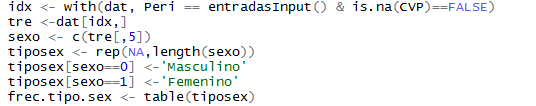
\includegraphics[scale=1]{algoritmo.png}
\caption{Algoritmo usado para filtrar la informaci\'on}
\end{figure}

Se implementaron   paneles  para dividir los diferentes gr\'aficos obtenidos.

Se implement\'o un gr\'afico de torta para sectorizar el g\'enero con respecto a los infectados con VIH. Se utilizo la siguiente funcion para su codificaci\'on.

\begin{figure}[H]
\centering
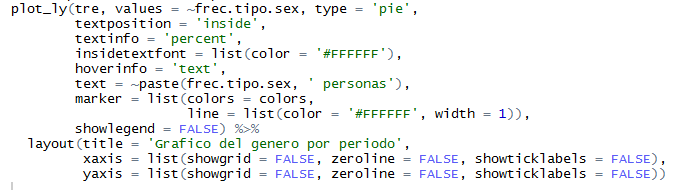
\includegraphics[scale=0.8]{torta.PNG}
\caption{Implementaci\'on en R del gr\'afico de torta}
\end{figure}

En la categor\'ia por la edad, se realiz\'o un histograma, y la debida implementacion del c\'odigo en R (Figura 4.7). Se realizo un filtro antes de realizar la graficaci\'on.

\begin{figure}[H]
\centering
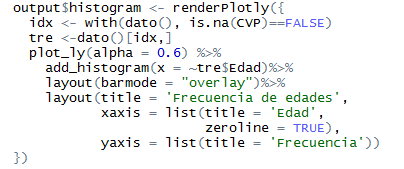
\includegraphics[scale=0.8]{histogram.PNG}
\caption{Implementaci\'on en R del histograma}
\end{figure}

En la categor\'ia por las cargas, para la mejor visualizaci\'on de los datos, se utiliz\'o un gr\'afico de puntos (Figura 4.8), las variables que son indispensables son la carga viral plasm\'atica, las c\'elulas $T^{+}CD4$ y $T^{+}CD8$. \\

\begin{figure}[H]
\centering
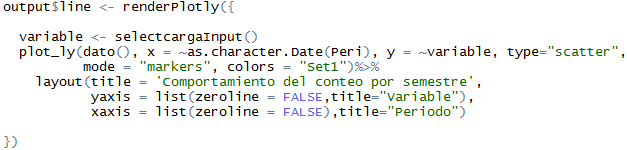
\includegraphics[scale=0.8]{ca.PNG}
\caption{Implementaci\'on en R de la selecci\'on de las cargas}
\end{figure}

Las limitaciones con respecto a la exploraci\'on de datos, son los datos faltantes, por lo cual, se aplicaron los debidos filtros para omitir dichos datos.\\

\subsection{Ajuste del modelo}

Se planific\'o la elaboraci\'on de los m\'odulos de Ajuste del m\'odelo y Validaci\'on del m\'odelo. El an\'alisis de las tendencias mostradas en los m\'odulos, se implement\'o mediante las librer\'ias de R, lm4, influence.ME, nlme y lmerTest.\\

En el m\'odulo Ajuste del m\'odelo, se realiz\'o el estudio de los datos longitudinales, las variables CVP, CD4 y CD8 son las utilizadas para aplicar el m\'odelo lineal mixto, cada paciente presenta varias m\'edidas de estas variables, con respecto a los años, las medidas  NA representan los datos faltantes, que indican que un  paciente decidio no ir mas al programa (patron mon\'otono)  o falta de forma intermitnte (patron no mon\'otono), esta es una de las razones que permite la utilizaci\'on de un modelo lineal de efectos mixtos, ya que esta t\'ecnica permite manejar, la alta heterogeneidad entre e intra pacientes, la correlaci\'on ente las medidas de un mismo paciente, as\'i como los datos faltantes.\\

Se emple\'o la formula del m\'odelo lineal mixto para hallar los valores asociados.

\begin{figure}[H]
\centering

\includegraphics[scale=1]{formula.png}
\caption{F\'ormula utilizada en el m\'odelo lineal mixto}
\end{figure}

El resultado de esta formula esta ajustado por REML.\\

\subsection{Validaci\'on del modelo}

El resultado gr\'afico corresponde a los resultados obtenidos en la formula de los modelos mixtos, y corresponde a la variaci\'on de los datos cargados en la aplicaci\'on (Figura 4.10).

\begin{figure}[H]
\centering
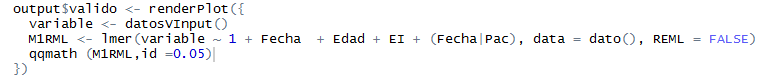
\includegraphics[scale=0.8]{validacion.PNG}
\caption{Implementaci\'on de los residuos de la validaci\'on del modelo}
\end{figure}
 
\subsection{Generaci\'on del reporte}

Se genero un archivo con extensi\'on .Rmd llamado reporte.Rmd, con la finalidad de crear el reporte en formato que se pueda guardar y el usuario pueda revisar y analizar los datos, se utilizo la siguiente estructura b\'asica para la generaci\'on del reporte (Figura 4.11).

\begin{figure}[H]
\centering
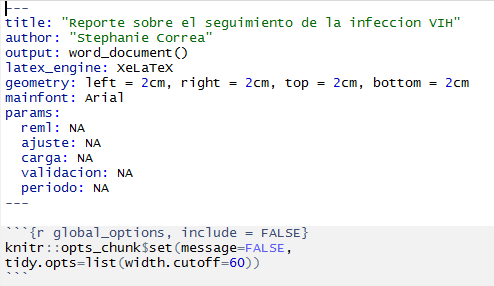
\includegraphics[scale=0.8]{reporte.PNG}
\caption{Estructura b\'asica del archivo reporte.Rmd}
\end{figure}

\subsection{Visualizaci\'on en el mapa}

Para la visualizaci\'on del mapa, se realizo la siguiente implementaci\'on de c\'odigo.

\begin{figure}[H]
\centering
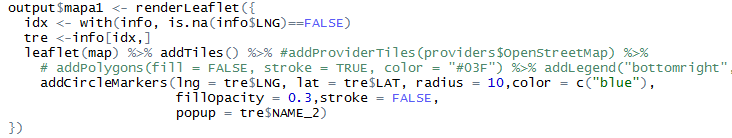
\includegraphics[scale=0.8]{mapa.PNG}
\caption{Implementaci\'on en R de la visualizaci\'on del mapa}
\end{figure}

 
En esta etapa se estableci\'o un plan de integraci\'on y pruebas, en caso de las pruebas unitarias, se realizaron en 2 fases, la primera con datos sint\'eticos que permitan comprobar cada estado del diagrama de flujo, que esquematiza la soluci\'on num\'erica que permite el c\'alculo de cada uno de los \'indices fisiol\'ogicos para entre otra herramientas pueden utilizarse los paquetes de R \emph{RUnit} \textit{\citet{runit}} y \emph{testthat} \citet{test}, y la segunda etapa donde cada funci\'on asociada a un \'indice fisiol\'ogico se le realizan prueban con los conjuntos de datos de prueba que formaran parte integral del paquete y con los cuales se desarrollaran los ejemplos pr\'acticos que conformaran la documentaci\'on que acompaña al paquete R.\\

\section{Etapa 4}
    
La etapa 4 esta compuesta  solo por 3 fases, ya que en esta etapa se ha obtenido el prototipo operativo, el cual se han implementado las diferentes pruebas de caja blanca y caja negra.\\

En la etapa anterior, se realiz\'o un plan de integraci\'on y pruebas, donde se estableci\'o la utilizaci\'on de las herramientas \textit{RUnit} y \textit{testthat}. \\

La implementaci\'on de la aplicaci\'on es la creaci\'on completa del paquete en R, donde el usuario puede descargar el paquete desde RStudio y utilizar la aplicaci\'on HIVmlm.

\begin{figure}[H]
\centering
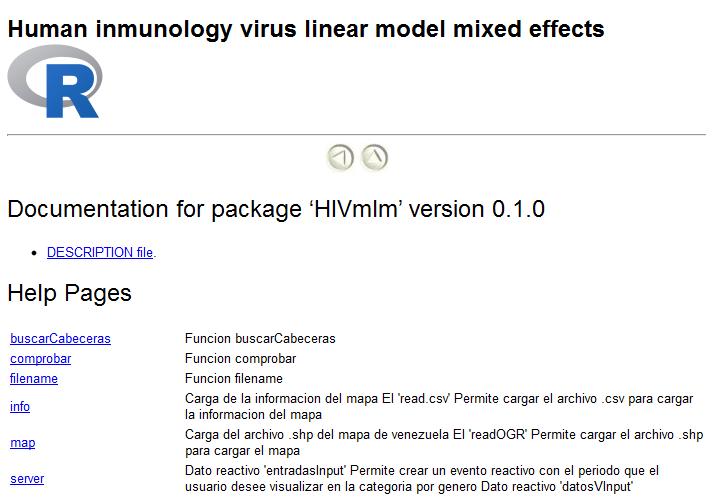
\includegraphics[scale=0.8]{HIVmlm.PNG}
\caption{Paquete cargado en las librerias de R}
\end{figure}








 

\chapter{Conclusiones y recomendaciones}

Se diagnostic\'o la informaci\'on obtenida de la base de datos que fue suministrada por el Instituto Aut\'onomo Hospital Universitario de los Andes, con el fin de filtrar los datos que all\'i estaban expuestos para preservar la identidad de los pacientes, y escoger los datos y variables que mejor se adaptaron al desarrollo de la aplicaci\'on. Para un mejor analisis de los resultados, se agruparon los pacientes por municipios del estado M\'erida, con el fin de realizar un mejor ubicaci\'on geoespacial, con la debida visualizaci\'on y representaci\'on en el mapa. \\

La base de datos una vez filtrada, permiti\'o analizar de manera exploratoria y descriptiva, la selecci\'on de las variables que se implementaron en el modelo; las cuales hicieron referencia a los diferentes resultados de las pruebas con respecto a la seroconversion del VIH, muestras de datos que el paciente se hace con regularidad, es decir, el conteo de la carga viral plasmatica, un dato relevante e indispensable para el modelo, as\'i como el conteo de las celulas $T^{+}CD4$ y  $T^{+}CD8$. Algunos datos que fueron tomados en cuenta para el analisis fueron los demogr\'aficos:  la edad, el genero, el periodo y el municipio donde reside el paciente para esta investigaci\'on se trabajo como caso de estudio el estado M\'erida. \\


Se implement\'o un modelo lineal mixto, porque es ampliamente utilizado en el analisis de datos longitudinales, especificamente en el \'area de la medicina en el seguimiento de cohortes de pacientes, además su implementaci\'on en R, permiti\'o que pueda estimarse en un ambiente WEB, sin el uso de recursos computacionales de altas prestaciones.\\

Se realizaron las debidas pruebas de funcionalidad a la aplicaci\'on en cada etapa de desarrollo de la metodologia, as\'i como tambi\'en las pruebas de caja blanca con las herramientas de R antes mecionadas en el capítulo 4, permitiendo demostrar su operatividad en el manejo de los fallos.\\

Finalmente, destaca su uso como herramienta de an\'alisis descriptivo de la incidencia del VIH en el estado M\'erida para el estudio de  datos de tipo  longitudinal, el cual por estar desarrollado con una herramienta en la que se trabaja bajo el esquema colaborativo, es una herramienta de fácil mantemiento y escalable, y aunque las pruebas de funcionabilidad se realizaron sólo considerando los marcadores inmunol\'ogicos y virol'ogicos disponibles en las vistas minables obtenidos en el filtrado de los datos, tambi\'en puede considerarse evaluar con el modelo lineal mixto, el impacto de las coinfecciones con otros virus, las condiciones de medicación, grupos de riesgo, entre otras variables.\\

\section{Recomendaciones}

Implementar el modelo a los diferentes estados del pa\'is, incluyendo las vistas minables del los otros estados que se encuentran almacenadas en la base de datos del Laboratorio de Investigaciones Hormonales del Instituto Aut\'onomo Hospital Universitario de los Andes.\\

Unificar esfuerzos con organismos de salud p\'ublicos y privados para el desarrollo de una aplicaci\'on que unifique tanto la incidencia del virus como hacer analisis predictivos de la misma.\\



 




\appendix
%% Cap'itulos incluidos despues del comando \appendix aparecen como ap'endices
%% de la tesis.
\chapter{Definici\'on de T\'erminos}

\textbf{Antirretroviral: } Medicamento empleado para impedir la multiplicaci\'on de un retrovirus, como el VIH. Por lo general, el t\'ermino se refiere a los medicamentos antirretrovirales contra el VIH.

\textbf{Carga viral: } Cantidad del VIH en una muestra de sangre. Se notifica como el n\'umero de copias de ARN del VIH por mil\'imetro de sangre. Una meta importante del tratamiento antirretroviral (TAR) es reducir la concentraci\'on de carga viral de una persona a un nivel indetectable, que es demasiado baja para detectar el virus con una prueba de la carga viral.

\textbf{Coinfecci\'on: } es un t\'ermino empleado cuando una persona tiene dos o m\'as enfermedades infecciosas a la vez. Puesto que es posible infectarse con VIH y hepatitis C (VHC o Hep C para abreviar) por las mismas v\'ias,  hasta 3 personas de cada 10 infectadas con el VIH est\'an infectadas tambi\'en con el VHC.

\textbf{Control de versiones: } Es la gesti\'on de los diversos cambios que se realizan sobre los elementos de alg\'un producto o una configuraci\'on del mismo, es decir, a la gesti\'on de los diversos cambios que se realizan sobre los elementos de alg\'un producto o una configuraci\'on.

\textbf{Comorbilidad: } Tambi\'en conocida como "morbilidad asociada", es un t\'ermino utilizado para describir dos o m\'as trastornos o enfermedades que ocurren en la misma persona. Pueden ocurrir al mismo tiempo o uno despu\'es del otro. La comorbilidad tambi\'en implica que hay una interacci\'on entre las dos enfermedades que puede empeorar la evoluci\'on de ambas.

\textbf{DESCRIPTION: } Archivo que contiene informaci\'on b\'asica sobre el paquete.

\textbf{Estudio longitudinal:} Es un tipo de diseño de investigaci\'on que consiste en estudiar y evaluar a las mismas personas por un per\'iodo prolongado de tiempo.

\textbf{Git: } Es un software de control de versiones diseñado por Linus Torvalds.

\textbf{GitHub: } Es una plataforma de desarrollo colaborativo de software para alojar proyectos utilizando el sistema de control de versiones Git.

\textbf{ggplot2:} El paquete ggplot2 de R proporciona un poderoso sistema que hace que sea f\'acil de producir gr\'aficos complejos de varias capas, automatiza varios aspectos tediosos del proceso de graficar manteniendo al mismo tiempo la habilidad de construir paso a paso un gr\'afico pues se compone de una serie de pequeños bloques de construcci\'on independientes, esto reduce la redundancia dentro del c\'odigo, y hace que sea f\'acil de personalizar el gr\'afico para obtener exactamente lo que se desea.

\textbf{IDE: } Una Infraestructura de Datos Espaciales (IDE) es un sistema de informaci\'n integrado por un conjunto de recursos (cat\'alogos, servidores, programas, datos, aplicaciones, p\'aginas Web,…) dedicados a gestionar Informaci\'on Geogr\'afica (mapas, ortofotos, im\'agenes de sat\'elite, top\'onimos,…), disponibles en Internet, que cumplen una serie de condiciones de interoperabilidad (normas, especificaciones, protocolos, interfaces,…), y que permiten que un usuario, utilizando un simple navegador, pueda utilizarlos y combinarlos seg\'un sus necesidades.

\textbf{influence.ME: } Calcula las medidas de influencia para m\'odelos de efectos mixtos estimados con lme4. El razonamiento b\'asico detr\'as de la medici\'on de casos influyentes, es que cuando se omiten iterativamente unidades individuales
a partir de los datos, los m\'odelos basados en estos datos no deber\'ian producir estimaciones sustancialmente diferentes. 

\textbf{ITS: } son enfermedades infecciosas, que pueden transmitirse de una persona a otra durante una relaci\'on sexual vaginal, anal u oral. Las ITS afectan a todos independientemente de la orientaci\'on sexual o identidad de g\'enero. Desde el comienzo de la vida sexual puede estar expuesto/a a estas infecciones. Las producen m\'as de 30 diferentes tipos de virus, bacterias y par\'asitos. Las m\'as frecuentes son la s\'ifilis, gonorrea, clamidia, herpes, hepatitis B y C, VIH y VPH.

\textbf{IAHULA: } Instituto aut\'onomo hospital universitario de los andes.

\textbf{Linfocito $T^{+}CD4$:} Los linfocitos (las c\'elulas) $T^{+}CD4$ ayudan a coordinar la respuesta inmunitaria al estimular a otros inmunocitos, como los macr\'ofagos, los linfocitos B y los linfocitos $T^{+}CD8$ para combatir la infecci\'on. El VIH debilita el sistema inmunitario al destruir los linfocitos CD4.

\textbf{Linfocito $T^{+}CD8$: } Los linfocitos (las c\'elulas) $T^{+}CD8$ reconocen y destruyen las c\'elulas infectadas por microorganismos, como bacterias o virus. 

\textbf{lme4: } Es un paquete de R que proporciona funciones para ajustar y analizar m\'odelos mixtos lineales, m\'odelos mixtos lineales generalizados y m\'odelos mixtos no lineales. En cada uno de estos nombres, el t\'ermino "mixto" o, m\'as completamente, "efectos mixtos", denota un m\'odelo que incorpora t\'erminos de efectos fijos y aleatorios en una expresi\'on predictiva a partir de la cual se puede evaluar la media condicional de la respuesta. 

\textbf{lmerTest: } Proporciona valores de p en anova de tipo I, II o III y tablas de resumen para ajustes del m\'odelo de lmer a trav\'es del m\'etodo de grados de libertad de Satterthwaite. Un m\'etodo de Kenward-Roger tambi\'en est\'a disponible a trav\'es del paquete pbkrtest. Los m\'etodos de selecci\'on de modelos incluyen tablas de pasos, drop1 y anova para efectos aleatorios (ranova). Tambi\'en están disponibles m\'etodos para medios m\'inimos cuadrados (LS-means) y pruebas de contrastes lineales de efectos fijos.

\textbf{M\'odelo lineal mixto: } Es una herramienta flexible para ajustar otros m\'odelos que se pueden formular como m\'odelos lineales mixtos. Dichos m\'odelos incluyen modelos multinivel, modelos lineales jer\'arquicos y modelos de coeficientes aleatorios.

\textbf{NAMESPACE: } Es una de las partes fundamentales de la construcci\'on de un paquete. Tener un NAMESPACE de alta calidad ayuda a encapsular el paquete y hacerlo aut\'onomo. Esto garantiza que otros paquetes no interfieran con el c\'odigo, que el c\'odigo no interfiera con otros paquetes y que el paquete funcione independientemente del entorno en el que se ejecute.

\textbf{nlme: } Ajusta y compara los m\'odelos gaussianos de efectos mixtos lineales y no lineales.

\textbf{Paquete R: } Es una colecci\'on de funciones, datos y c\'odigo R que se almacenan en una carpeta conforme a una estructura bien definida, f\'acilmente accesible para R.

\textbf{plotly: } Es una biblioteca gr\'afica de R, hace gr\'aficos interactivos de calidad de publicaci\'on en l\'inea. Ejemplos de c\'omo hacer gr\'aficos de l\'ineas, diagramas de dispersi\'on, gr\'aficos de \'areas, gr\'aficos de barras, barras de error, diagramas de cajas, histogramas, mapas de calor, subtramas, gr\'aficos de ejes m\'ultiples y gr\'aficos 3D (basados en WebGL).

\textbf{R: } Es un lenguaje orientado a objetos, el c\'alculo estad\'istico y la generaci\'on de gr\'aficos, que ofrece una gran variedad de t\'ecnicas estad\'isticas y gr\'aficas. Es un entorno de an\'alisis y programaci\'on estad\'isticos que, en su aspecto externo, es similar a S. Es un lenguaje de programaci\'on completo con el que se añaden nuevas t\'ecnicas mediante la definici\'on de funciones.

\textbf{Reactividad: } Cuando una entrada (input) cambia, el servidor reconstruye cada salida (output) que depende de ella (tambi\'en si la dependencia es indirecta).

\textbf{REML: } M\'axima verosimilitud restringida.

\textbf{Retrovirus: } Tipo de virus que emplea el ARN como su material gen\'etico. Despu\'es de infectar una c\'elula, un retrovirus emplea una enzima llamada transcriptasa inversa para convertir el ARN en ADN. Luego, el retrovirus integra su ADN en el ADN de la c\'elula huésped, que le permite multiplicarse. El VIH, causante del SIDA, es un retrovirus.

\textbf{RStudio: } Es una interfaz que permite acceder de manera sencilla a toda la potencia de R, para utilizar RStudio se requiere haber instalado R previamente.

\textbf{Seroconversi\'on: } Transici\'on de la infecci\'on por el VIH a la presencia detectable de anticuerpos contra ese virus en la sangre. Cuando ocurre seroconversi\'on (por lo general, a las pocas semanas de la infecci\'on), el resultado de una prueba de detecci\'on de anticuerpos contra el VIH cambia de seronegativo a seropositivo.

\textbf{Shiny: } Es una herramienta para crear f\'acilmente aplicaciones web interactivas (apps) que permiten a los usuarios interactuar con sus datos sin tener que manipular el c\'odigo.

\textbf{SIDA: } Es la enfermedad que se desarrolla como consecuencia de la destrucci\'on progresiva del sistema inmunitario (de las defensas del organismo), producida por un virus descubierto en 1983 y denominado Virus de la Inmunodeficiencia Humana (VIH). La definen alguna de estas afecciones: ciertas infecciones, procesos tumorales, estados de desnutrici\'on severa o una afectaci\'on importante de la inmunidad. La palabra SIDA proviene de las iniciales de S\'indrome de Inmunodeficiencia Adquirida, que consiste en la incapacidad del sistema inmunitario para hacer frente a las infecciones y otros procesos patol\'ogicos. El SIDA no es consecuencia de un trastorno hereditario, sino resultado de la exposici\'on a una infecci\'on por el VIH, que facilita el desarrollo de nuevas infecciones oportunistas, tumores y otros procesos. Este virus permanece latente y destruye un cierto tipo de linfocitos, c\'elulas encargadas de la defensa del sistema inmunitario del organismo.
 
\textbf{VIH: } El virus de la inmunodeficiencia humana (VIH) infecta a las c\'elulas del sistema inmunitario, alterando o anulando su funci\'on. La infecci\'on produce un deterioro progresivo del sistema inmunitario, con la consiguiente "inmunodeficiencia". Se considera que el sistema inmunitario es deficiente cuando deja de poder cumplir su funci\'on de lucha contra las infecciones y enfermedades. El s\'indrome de inmunodeficiencia adquirida (SIDA) es un t\'ermino que se aplica a los estadios m\'as avanzados de la infecci\'on por VIH y se define por la presencia de alguna de las m\'as de 20 infecciones oportunistas o de c\'anceres relacionados con el VIH. El VIH puede transmitirse por las relaciones sexuales vaginales, anales u orales con una persona infectada, la transfusi\'on de sangre contaminada o el uso compartido de agujas, jeringuillas u otros instrumentos punzantes. Asimismo, puede transmitirse de la madre al hijo durante el embarazo, el parto y la lactancia.

\textbf{Wireframe: } Un wireframe o prototipo no es m\'as que un boceto donde se representa visualmente, de una forma muy sencilla y esquem\'atica la estructura de una p\'agina web.
    

\chapter{Manual de usuario}

\textbf{Pantalla de inicio de HIVmlm}
\begin{figure}[H]
\centering
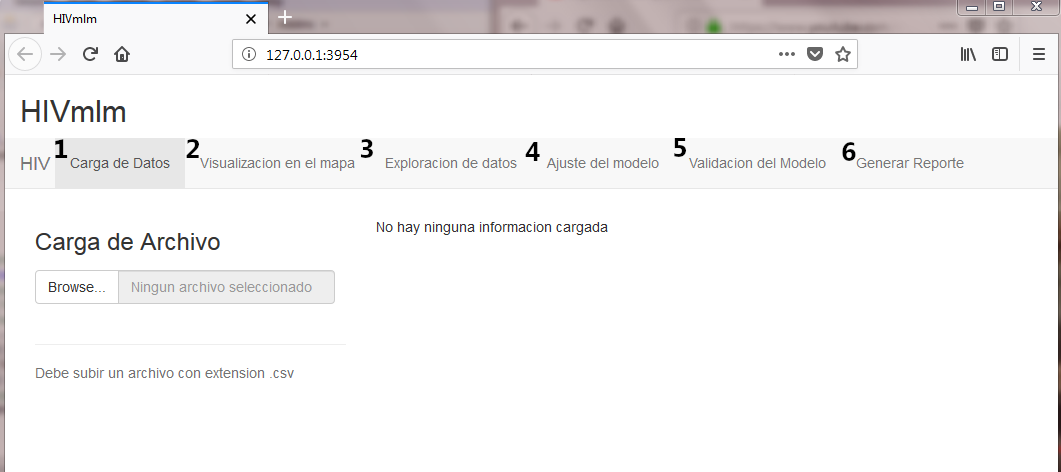
\includegraphics[scale=0.5]{inicio.PNG}
\caption{Pantalla de inicio de HIVmlm}
\end{figure}

\begin{enumerate}
\item \textbf{Carga de datos:} Modulo de carga del archivo
\item \textbf{Visualizaci\'on en el mapa:} Muestra la incidencia del virus en el mapa
\item \textbf{Exploraci\'on de datos:} Muestra el analisis grafico de los datos cargados
\item \textbf{Ajuste del Modelo:} Analisis del modelo lineal mixto
\item \textbf{Validaci\'on del modelo:} Muestra graficamente los datos obtenidos del modelo lineal mixto.
\item \textbf{Generar reporte:} Permite generar reportes con los datos de la aplicaci\'on 
\end{enumerate}

 \noindent
\textbf{M\'odulo de carga de datos}

\begin{figure}[H]
\centering
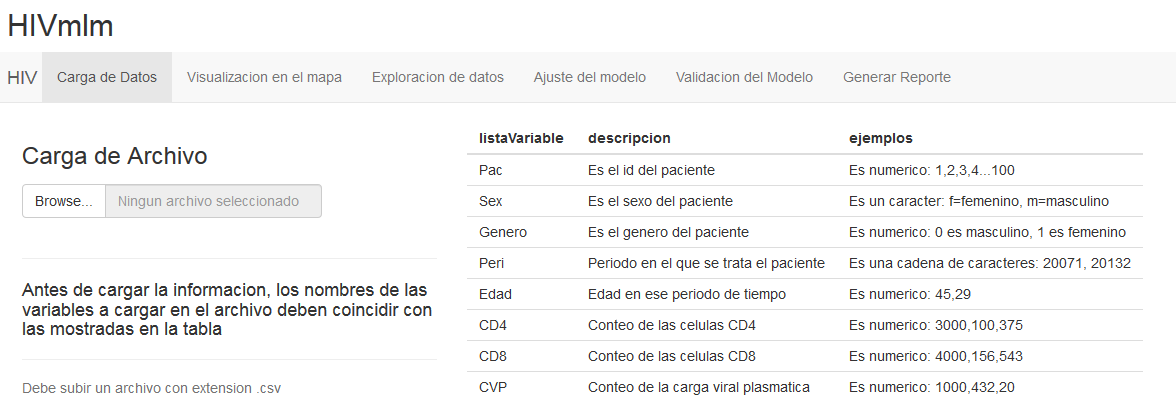
\includegraphics[scale=0.5]{cargaArchivo.PNG}
\caption{Pantalla de la carga del archivo}
\end{figure}

 \noindent
\textbf{Carga de datos}

Para cargar el archivo, se debe hace click en \textbf{Browse} como lo muestra la figura B.3.

\begin{figure}[H]
\centering
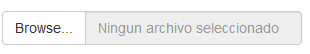
\includegraphics[scale=0.8]{browse.PNG}
\caption{Carga de archivo en la aplicaci\'on}
\end{figure}

Posteriormente se mostrar\'a una ventana para seleccionar el archivo como se muestra en la figura B.4.

\begin{figure}[H]
\centering
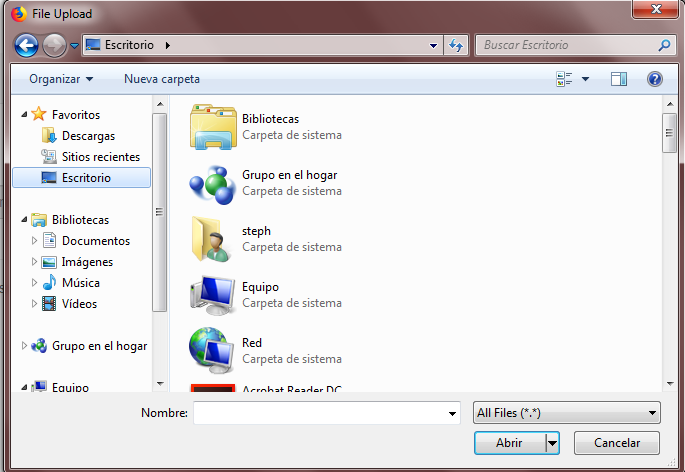
\includegraphics[scale=0.5]{fileup.PNG}
\caption{Selecci\'on del archivo a cargar}
\end{figure}

Se mostrar\'a la informaci\'on en la aplicaci\'on.

\begin{figure}[H]
\centering
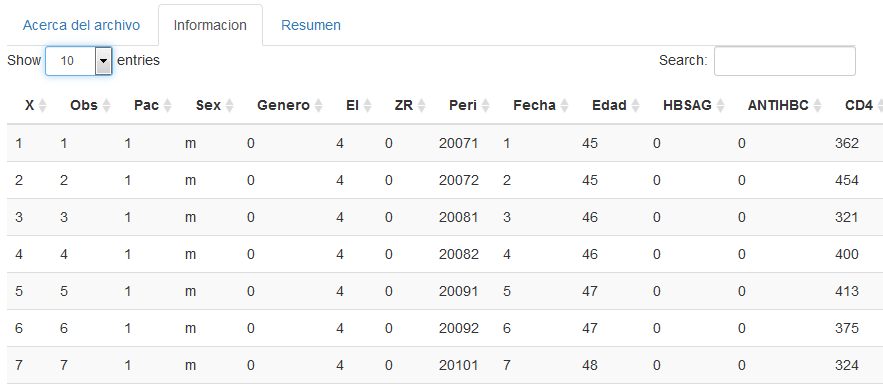
\includegraphics[scale=0.6]{Cargafile2.PNG}
\caption{Informaci\'on del archivo}
\end{figure}

Luego se puede navegar en la aplicaci\'on, con los diferentes modulos, para la exploraci\'on y el analisis de los datos.\\

 \noindent
\textbf{M\'odulo de visualizaci\'on del mapa}

En este m\'odulo, se detalla en el mapa, la incidencia de la ubicaci\'on y el contagio del virus en la localidad.

\begin{figure}[H]
  \centering
  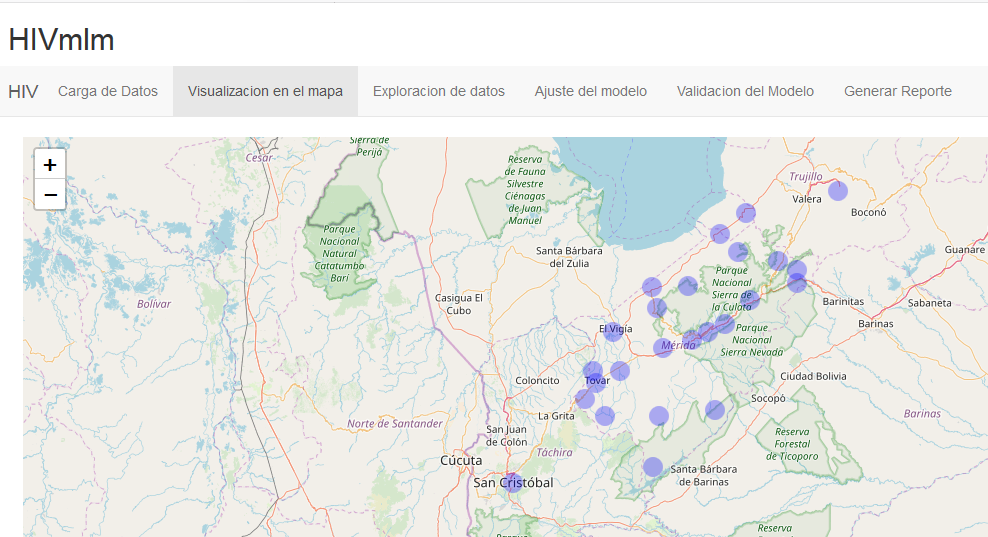
\includegraphics[scale=0.6]{mapa1.PNG}
   \caption{Pantalla de la visualizaci\'on del mapa}
  \end{figure}
  
Al presionar o darle click a los puntos azules ubicados en el mapa, se puede visualizar la informaci\'on realtiva a la media de la carga viral plasmatica y las c\'elulas CD4, n\'umero de pacientes, g\'enero, desviaci\'on estandar y tiempo medio de duraci\'on.

\begin{figure}[H]
\centering
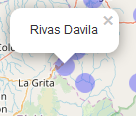
\includegraphics[scale=0.8]{mapa2.PNG}
\caption{Selecci\'on de un punto azul sobre el mapa}
\end{figure}

\textbf{M\'odulo de Exploraci\'on de datos}

En el siguiente m\'odulo, esta dividido en 3 paneles, es decir, el genero, la edad y las cargas. 

\begin{figure}[H]
\centering
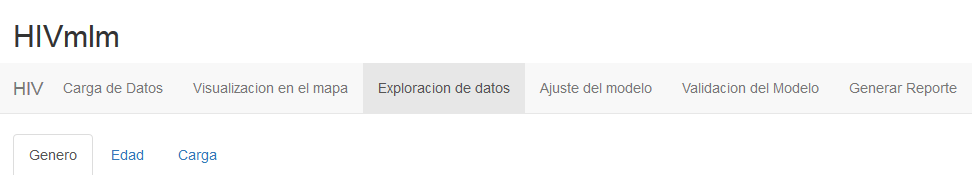
\includegraphics[scale=0.6]{explorar.PNG}
\caption{Visualizaci\'on del m\'odulo de Exploraci\'on de datos}
\end{figure}

En la siguiente figura, se puede visualizar que en la secci\'on \textbf{g\'enero} hay un selector por per\'iodo, en este caso, se puede seleccionar entre 20071 hasta 20132, obteniendo el siguiente gr\'afico.

\begin{figure}[H]
\centering
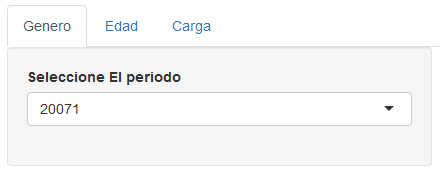
\includegraphics[scale=0.6]{panel.PNG}
\caption{Pantalla de los 3 paneles para visualizar graficamente los datos}
\end{figure}

\begin{figure}[H]
\centering
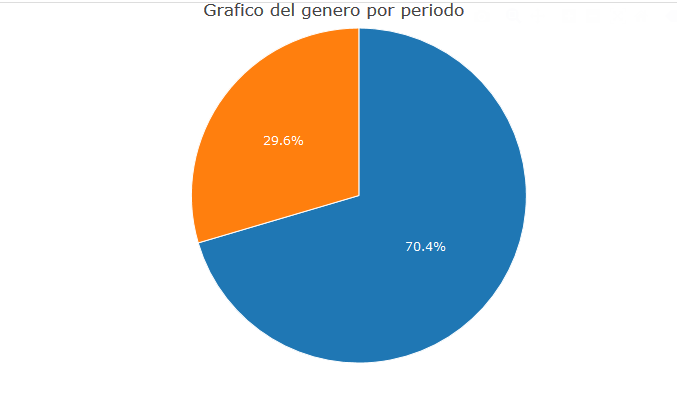
\includegraphics[scale=0.6]{genero.PNG}
\caption{Visualizaci\'on de la gr\'afica de torta por g\'enero}
\end{figure}

En la secci\'on \textbf{Edad} muestra un histograma como lo muestra la siguiente figura B.11

\begin{figure}[H]
\centering
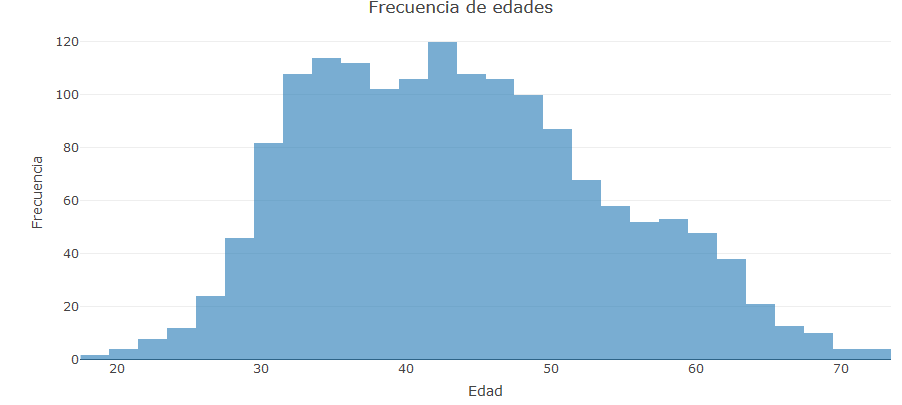
\includegraphics[scale=0.6]{edad.PNG}
\caption{Pantalla con el histograma de edades}
\end{figure}

En la secci\'on \textbf{Cargas} muestra un selector, con las variables Carga Viral plasmatica, celulas $T^{+}CD4$ y $T^{+}CD8$. Permite visualizar un gr\'afico de puntos.

\begin{figure}[H]
\centering
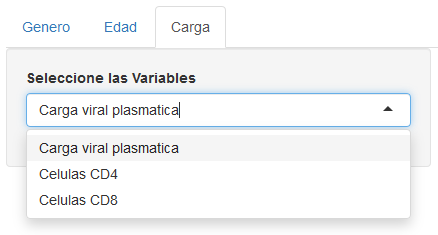
\includegraphics[scale=0.6]{exploraCarg.PNG}
\caption{Pantalla del selector de la secci\'on cargas}
\end{figure}

\begin{figure}[H]
\centering
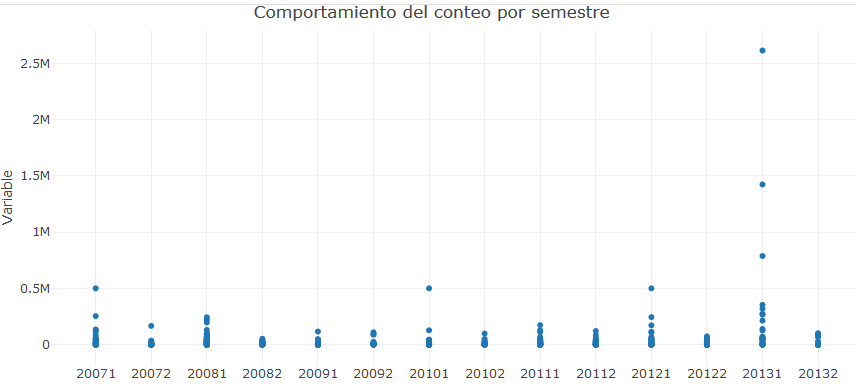
\includegraphics[scale=0.6]{CVP.PNG}
\caption{Visualizaci\'on del gr\'afico de puntos}
\end{figure}

 \noindent
\textbf{M\'odulo Ajuste del modelo}

En este m\'odulo, muestra la implementaci\'on del modelo lineal mixto.

\begin{figure}[H]
\centering
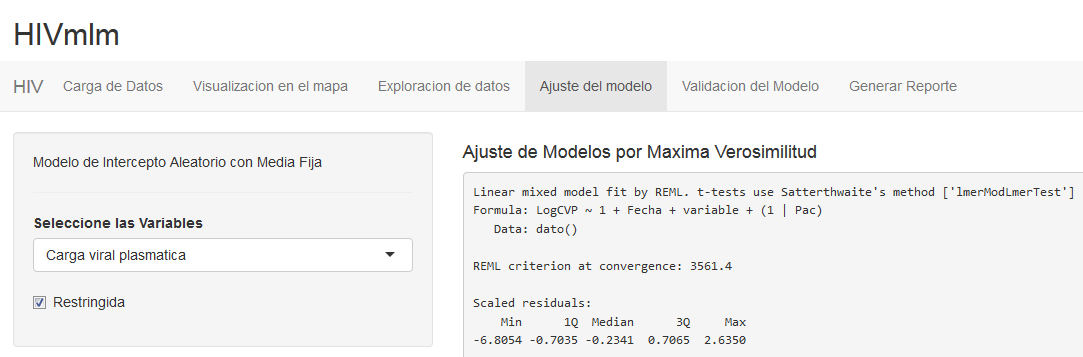
\includegraphics[scale=0.5]{ajusteModel.PNG}
\caption{Pantalla con el m\'odulo ajuste del modelo}
\end{figure}

Contiene un selector que permite seleccionar entre las variables carga viral plasm\'atica, c\'elulas $T^{+}CD4$ y $T^{+}CD8$ y un cuadro de selecci\'on, con la variable Restingida, permitiendo variar el modelo matem\'atico.

\begin{figure}[H]
\centering
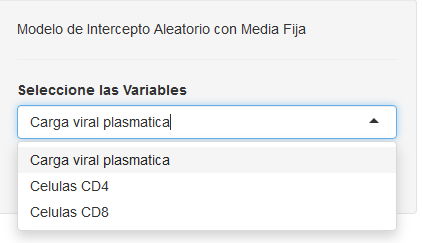
\includegraphics[scale=0.6]{cuadrosele.PNG}
\caption{Pantalla con el selector del m\'odulo de ajuste del modelo}
\end{figure}

Luego de seleccionar las variables, sale la siguiente informaci\'on como lo muestra la figura B.16.

\begin{figure}[H]
\centering
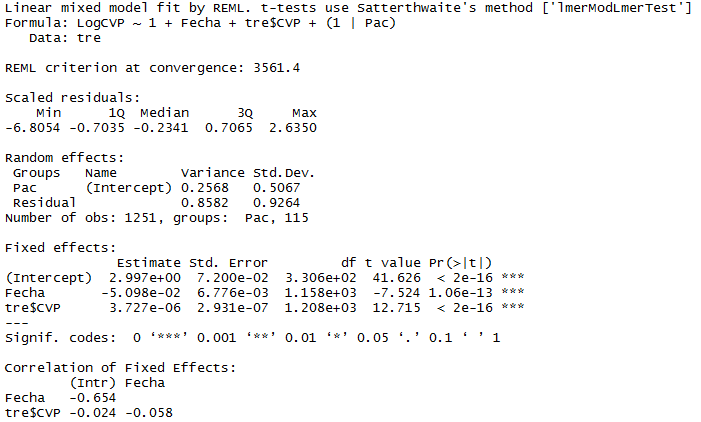
\includegraphics[scale=0.6]{lme.png}
\caption{Pantalla con la informaci\'on del modelo lineal mixto}
\end{figure}

 \noindent
\textbf{M\'odulo de validaci\'on del modelo}

En este m\'odulo, muestra el resultado de los residuos, calculados en el m\'odulo anterior, el ajuste del modelo, lo que permite visualizar el comportamiento de los datos en el modelo lineal mixto. Permite seleccionar entre las variables Carga viral plasmatica, celulas $T^{+}CD4$ y $T^{+}CD8$.

\begin{figure}[H]
\centering
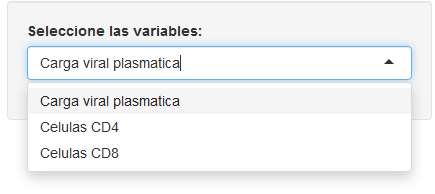
\includegraphics[scale=0.6]{valido2.PNG}
\caption{Pantalla selecci\'on de las variables de la validaci\'on del modelo}
\end{figure}

Genera la siguiente gr\'afica.

\begin{figure}[H]
\centering
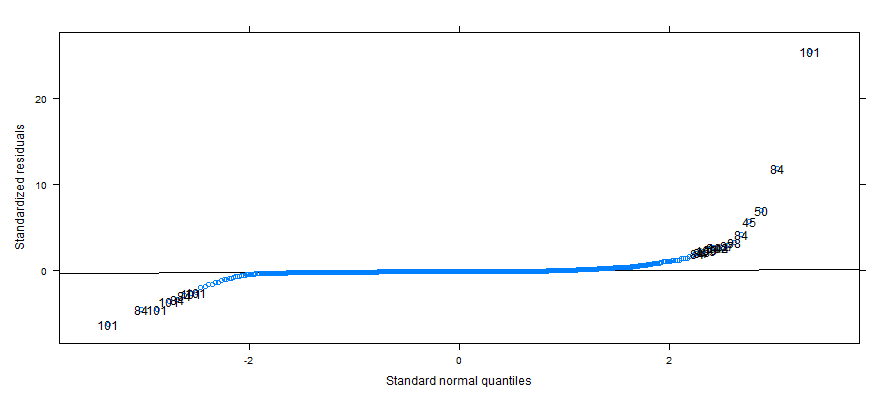
\includegraphics[scale=0.6]{valido.PNG}
\caption{Gr\'afica de la validaci\'on del modelo}
\end{figure}

\textbf{M\'odulo generar reporte}

En este m\'odulo, permite generar el reporte de las graficas y el an\'alisis del modelo lineal mixto. Aparece un boton de descargar reporte, se le da click.

\begin{figure}[H]
\centering
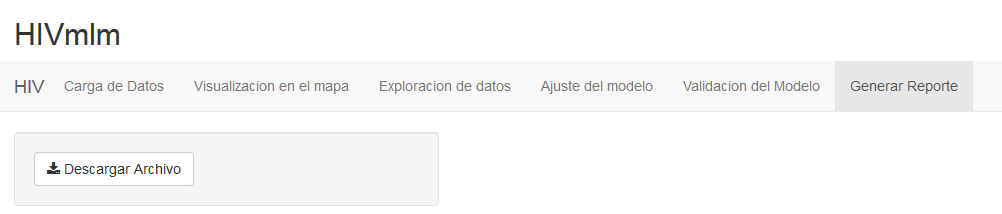
\includegraphics[scale=0.6]{reporte2.PNG}
\caption{Pantalla del bot\'on de descarga del reporte}
\end{figure}

Luego aparece una ventana, donde permite guardar el reporte, se le da click en ok, y lo guarda.

\begin{figure}[H]
\centering
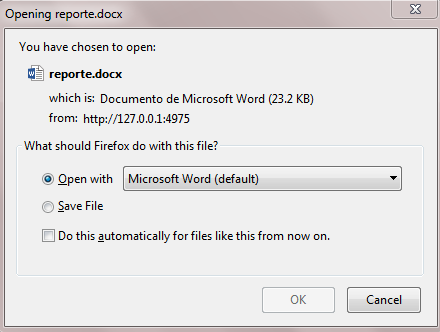
\includegraphics[scale=0.6]{reporte3.PNG}
\caption{Pantalla de guardar el reporte}
\end{figure}









    


%\include{apendiceC}

%% Incluir la bibliograf'ia. Mirar el archivo "biblio.bib" para m'as detales
%% y un ejemplo.
\bibliographystyle{apalike}
\bibliography{biblio}


\end{document}
